\documentclass[11pt,a4paper]{article}
\usepackage[utf8]{inputenc}
\usepackage[T1]{fontenc}
\usepackage{lmodern}
\usepackage[margin=2.4cm,headheight=15pt]{geometry}
\usepackage{xcolor,booktabs,array,tabularx,longtable,enumitem,graphicx,listings,fancyhdr,hyperref,tikz}
\usetikzlibrary{arrows.meta,positioning,fit,shapes.geometric}
\definecolor{navy}{HTML}{18354B}
\definecolor{bluebg}{HTML}{EAF2FA}
\hypersetup{colorlinks=true,linkcolor=navy,urlcolor=navy,pdftitle={Laporan Akhir EventKu Kelompok IV (UTS dan UAT)}}
\pagestyle{fancy}\fancyhf{}\fancyhead[L]{\small EventKu -- Laporan Akhir}\fancyhead[R]{\small Kelompok IV}\fancyfoot[C]{\thepage}
\setlength{\parindent}{0pt}\setlength{\parskip}{7pt}\setlength{\emergencystretch}{3em}
\renewcommand{\contentsname}{Daftar Isi}\renewcommand{\refname}{Referensi}
\setlist{nosep,leftmargin=*,topsep=4pt}
\widowpenalty=10000\clubpenalty=10000
\renewcommand{\arraystretch}{1.2}
\newcolumntype{Y}{>{\raggedright\arraybackslash}X}
\newcommand{\tbl}[2]{\par\smallskip\noindent\begin{tabularx}{\linewidth}{#1}\toprule #2\bottomrule\end{tabularx}\par\smallskip}
\newcommand{\note}[1]{\par\smallskip\noindent\fcolorbox{navy}{bluebg}{\parbox{\dimexpr\linewidth-2\fboxsep-2\fboxrule\relax}{\small #1}}\par\smallskip}
\newcommand{\page}[1]{\clearpage\section{#1}}
\tikzset{box/.style={draw=navy,rounded corners,fill=bluebg,align=center,text width=3cm,minimum height=1cm,font=\small},arr/.style={-{Stealth},draw=navy},uc/.style={ellipse,draw=navy,fill=bluebg,align=center,text width=3cm,minimum height=.9cm,font=\small}}
\lstset{basicstyle=\ttfamily\small,breaklines=true,frame=single,backgroundcolor=\color{bluebg},columns=fullflexible,keepspaces=true,showstringspaces=false}
\newcommand{\lucidfig}[3]{\par\begin{center}\includegraphics[width=\linewidth,height=#2,keepaspectratio]{figures/#1.png}\par\small #3\par\footnotesize Sumber: ekspor Lucidchart versi revisi dalam DOCX kelompok. \url{https://lucid.app/lucidchart/eade4b94-4f0b-4ff1-9576-4063f45cfbfb/view?invitationId=inv_144411dc-3a44-4e55-8ed9-8ea69347d77b&page=index}.\end{center}\par}
\newcommand{\uifig}[3]{\par\begin{center}\includegraphics[width=\linewidth,height=#2,keepaspectratio]{figures/figma/#1.png}\par\small #3\par\footnotesize Sumber: rancangan Figma Audrey, pada DOCX wireframe dan UI high-fidelity Minggu 7.\end{center}\par}
\newcommand{\contribfig}[3]{\par\begin{center}\begin{minipage}{\linewidth}\centering\includegraphics[width=\linewidth,height=#2,keepaspectratio]{figures/kontribusi/alexa/bukti_#1.png}\par\small #3\par\footnotesize Sumber: lampiran jawaban individu Alexa.\end{minipage}\end{center}\par}
\newcommand{\bambangexport}[3]{\par\begin{center}\includegraphics[width=\linewidth,height=#2,keepaspectratio]{figures/kontribusi/bambang/lucidchart_#1.png}\par\small #3\par\footnotesize Sumber: PNG ekspor Lucidchart yang disampaikan Bambang; versi awal sebelum penyelarasan SRS. \url{https://lucid.app/lucidchart/eade4b94-4f0b-4ff1-9576-4063f45cfbfb/view?invitationId=inv_144411dc-3a44-4e55-8ed9-8ea69347d77b&page=index}.\end{center}\par}
\begin{document}
\hypersetup{pageanchor=false}
\begin{titlepage}
\thispagestyle{empty}
\fontfamily{ptm}\fontsize{12}{15}\selectfont\color{black}
\null
\begin{tikzpicture}[remember picture,overlay]
\node[anchor=center,align=center,text width=\linewidth,inner sep=0pt,font=\bfseries]
  at ([yshift=-3.35cm]current page.north)
  {LAPORAN AKHIR REKAYASA PERANGKAT LUNAK (UTS DAN UAT)};
\node[anchor=center,align=center,text width=\linewidth,inner sep=0pt,font=\bfseries]
  at ([yshift=-4.85cm]current page.north)
  {EVENTKU -- SISTEM INFORMASI DAN PENDAFTARAN EVENT KAMPUS};
\node[anchor=center,inner sep=0pt]
  at ([yshift=-11cm]current page.north)
  {
\includegraphics[height=8.7cm,trim=105bp 57bp 105bp 57bp,clip]{figures/logowm.png}};
\node[anchor=center,inner sep=0pt,font=\bfseries]
  at ([yshift=-17.2cm]current page.north)
  {ANGGOTA TIM};
\node[anchor=north,inner sep=0pt,align=left]
  at ([yshift=-17.9cm]current page.north)
  {\renewcommand{\arraystretch}{1.05}%
   \begin{tabular}{@{}p{7.3cm}l@{}}
   Audrey Elizabeth Gracesia & 5803024014\\
   Bambang Herlambang & 5803024019\\
   Dustin Pranata Wangsawidjaja & 5803024021\\
   Alexa Bilxiz Aulia & 5803024023\\
   \end{tabular}};
\node[anchor=north,align=center,text width=\linewidth,inner sep=0pt,font=\bfseries]
  at ([yshift=-22.8cm]current page.north)
  {PROGRAM STUDI INFORMATIKA\\[.3cm]
   FAKULTAS TEKNIK\\[.3cm]
   UNIVERSITAS KATOLIK WIDYA MANDALA\\[.3cm]
   SURABAYA\\[.3cm]
   2026};
\end{tikzpicture}
\end{titlepage}
\hypersetup{pageanchor=true}
{\small\setlength{\parskip}{0pt}\tableofcontents}
\page{Identitas dan Deskripsi Proyek}
EventKu adalah aplikasi web untuk memusatkan informasi kegiatan kampus dan pendaftaran peserta. Laporan ini menggabungkan analisis kebutuhan dan rancangan kelompok sampai tahap UTS. SRS versi 2 menjadi acuan kebutuhan; Figma merupakan artefak visual yang belum mencakup seluruh kebutuhan.
\subsection{Pembagian Peran}
\tbl{p{3.6cm}p{3cm}Y}{Nama & Peran & Tanggung jawab\\\midrule
Audrey Elizabeth Gracesia & Backend dan UI/UX & Rancangan API, alur backend, wireframe dan antarmuka.\\
Bambang Herlambang & System Architect dan Frontend & ERD, arsitektur modular, class diagram, pattern dan frontend.\\
Dustin Pranata Wangsawidjaja & PM dan Business Analyst & Charter, SDLC, SRS, backlog dan koordinasi.\\
Alexa Bilxiz Aulia & QA dan DevOps & Rancangan pengujian, kualitas, kolaborasi dan deployment.\\}
\subsection{Latar Belakang}
Informasi seminar, lomba, workshop, dan kegiatan organisasi tersebar melalui poster, grup percakapan, dan media sosial. Mahasiswa perlu memeriksa banyak saluran untuk mengetahui jadwal, lokasi, serta pendaftaran. Penyelenggara membutuhkan pencatatan peserta yang konsisten dengan kapasitas kegiatan.
Pemusatan informasi membantu mahasiswa menemukan kegiatan sesuai minat dan membantu penyelenggara memantau peserta. Moderasi admin diperlukan agar katalog publik hanya menampilkan kegiatan yang disetujui.
\subsection{Masalah Utama}
\begin{itemize}
\item Informasi kegiatan sulit ditelusuri berdasarkan jadwal atau kategori.
\item Pendaftaran terpisah dari informasi dan berisiko duplikasi atau melebihi kuota.
\item Penyelenggara memerlukan status publikasi, daftar peserta, dan ekspor data.
\item Pengelolaan organisasi dan publikasi memerlukan aturan akses yang jelas.
\end{itemize}
\page{Tujuan, Ruang Lingkup, dan Batasan}
\tbl{p{4cm}Y}{Tujuan & Bukti keberhasilan yang perlu diperoleh\\\midrule
Memudahkan pencarian & Kata kunci, kategori, tanggal, penyelenggara menghasilkan daftar event Disetujui.\\
Menertibkan pendaftaran & Satu pendaftaran aktif per mahasiswa per event; kuota tidak terlampaui pada permintaan bersamaan.\\
Menjaga kualitas publikasi & Event melewati pengajuan dan moderasi; penolakan memuat alasan.\\
Membantu penyelenggara & Peserta dan ekspor CSV sesuai lingkup organisasi serta hak akses.\\
Memudahkan penggunaan & Responsif minimal 360 piksel, bahasa Indonesia; pencarian--RSVP ditargetkan maksimal lima klik.\\}
\subsection{Lingkup MVP}
\begin{enumerate}
\item Registrasi, login, logout, JWT, dan otorisasi mahasiswa, penyelenggara, admin.
\item Verifikasi organisasi sebelum pengajuan kegiatan.
\item Draft, pengajuan, moderasi, pengelolaan event dan katalog publik.
\item Pencarian, filter gabungan, detail dan kalender bulanan.
\item RSVP, pembatalan sebelum mulai, riwayat dan kontrol kuota atomik.
\item Minat kategori, daftar notifikasi dan pemberitahuan event baru.
\item Dashboard, daftar peserta, ekspor CSV dan pengelolaan kategori.
\end{enumerate}
\subsection{Batasan}
Aplikasi native, tiket berbayar, dan integrasi SSO kampus berada di luar MVP. Bookmark, rating, dan beberapa notifikasi tambahan mengikuti prioritas Should/Could serta kapasitas tim. Proyek berlangsung 16 minggu dengan empat anggota. Data demonstrasi perlu disiapkan sebagai data uji.
Laporan ini tidak menyatakan sistem telah berjalan di produksi atau target performa telah tercapai. PostgreSQL ditetapkan sebagai database relasional. Persetujuan pemangku kepentingan dan hasil pengujian aktual tetap perlu dikonfirmasi tim.
\page{SDLC dan Posisi Proyek}
\subsection{Scrum yang Diadaptasi untuk Perkuliahan}
Dokumen justifikasi memilih Scrum karena kebutuhan dapat berkembang, risiko integrasi perlu diketahui lebih awal, dan implementasi dapat dibagi menjadi increment. Tim memakai backlog MoSCoW dan merencanakan planning, review, serta retrospective.
Analisis dan rancangan awal dilakukan sebelum UTS, sedangkan standup direncanakan mengikuti ketersediaan tim. Ini adaptasi untuk perkuliahan, bukan bukti bahwa seluruh praktik Scrum resmi sudah diterapkan. Scrum menggunakan pendekatan iteratif dan inkremental serta inspeksi dan adaptasi \cite{scrum}.
\begin{center}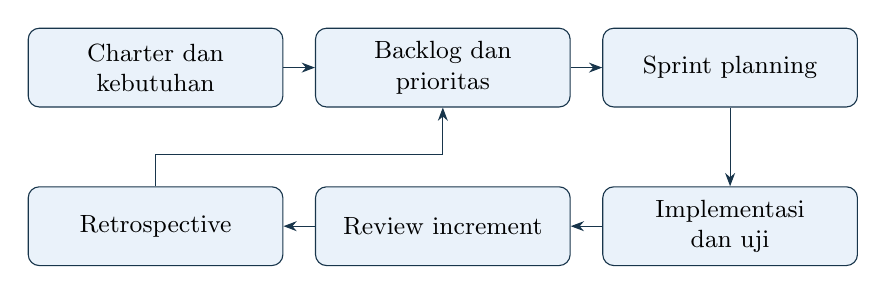
\begin{tikzpicture}[node distance=.4cm]
\node[box] (a) {Charter dan kebutuhan};\node[box,right=of a] (b) {Backlog dan prioritas};\node[box,right=of b] (c) {Sprint planning};
\node[box,below=1cm of c] (d) {Implementasi dan uji};\node[box,left=of d] (e) {Review increment};\node[box,left=of e] (f) {Retrospective};
\draw[arr] (a)--(b);\draw[arr] (b)--(c);\draw[arr] (c)--(d);\draw[arr] (d)--(e);\draw[arr] (e)--(f);\draw[arr] (f.north)--++(0,.4)-|(b.south);
\end{tikzpicture}\par\small Gambar 1. Siklus pengembangan yang direncanakan.\end{center}
\tbl{p{2.6cm}p{1.7cm}Y}{Tahap & Minggu & Artefak/rencana\\\midrule
Inisiasi & 1 & Identitas, masalah, peran, charter.\\
Analisis & 2--4 & SRS, user story, backlog dan prioritas.\\
Perancangan & 5--7 & Activity diagram, ERD, arsitektur, UML, Figma dan pattern.\\
Evaluasi UTS & 8 & Konsolidasi laporan dan evaluasi kesiapan.\\
Implementasi & 9--13 & Increment aplikasi dan pengujian tiap sprint.\\
Validasi akhir & 14--16 & Pengujian sistem, UAT, deployment, dokumentasi.\\}
Artefak rancangan tersedia; ketersediaannya tidak membuktikan review, persetujuan, atau implementasi fitur telah selesai.
\page{Perbandingan SDLC dan Pengendalian Iterasi}
Penilaian berikut berasal dari justifikasi internal tim. Skala 1--5 menunjukkan kesesuaian dengan konteks proyek, bukan pengukuran independen.
\tbl{Yrrrr}{Kriteria & Bobot & Waterfall & Iteratif & Scrum\\\midrule
Adaptasi perubahan & 5 & 1 & 4 & 5\\
Deteksi risiko dini & 5 & 2 & 4 & 5\\
Waktu 16 minggu & 4 & 3 & 3 & 4\\
Transparansi kemajuan & 4 & 3 & 3 & 5\\
Tim kecil & 3 & 3 & 4 & 5\\
Dokumentasi & 4 & 5 & 3 & 3\\
Kemudahan bagi pemula & 3 & 4 & 3 & 3\\\midrule
Total berbobot & 28 & 80 & 97 & 122\\}
\subsection{Kelebihan dan Keterbatasan}
Waterfall menyediakan urutan dan dokumentasi jelas, tetapi perubahan kebutuhan dapat memerlukan revisi lintas tahap. Model iteratif memungkinkan penyempurnaan bertahap; prioritas dan penilaian increment tetap diperlukan. Scrum mendukung transparansi backlog dan review rutin, tetapi memerlukan komitmen, kapasitas yang realistis, serta definisi selesai terukur.
\subsection{Pengendalian Perubahan}
Perubahan dicatat dengan ID kebutuhan, alasan, dampak pada diagram/API, dan estimasi. PM/BA mengelola prioritas bersama tim. Must didahulukan; Should/Could tidak boleh mengorbankan integritas kuota, otorisasi dan moderasi.
\note{Dokumen awal menyebut tiga sprint sekitar dua minggu pada Minggu 9--13, sedangkan rentang ini hanya lima minggu. Usulan konsisten: Sprint 1 Minggu 9--10, Sprint 2 Minggu 11--12, Sprint 3 Minggu 13. Ini perlu disepakati tim.}
Definition of Ready memastikan kebutuhan dan penerimaan dipahami. Definition of Done disarankan mencakup review kode, pengujian relevan, pembaruan dokumentasi/API, dan demonstrasi increment. Bukti pelaksanaannya baru dapat dilaporkan setelah aktivitas tersebut berlangsung.
\page{Pemangku Kepentingan dan Kebutuhan Fungsional}
\tbl{p{3cm}Yp{3.4cm}}{Pihak & Kebutuhan & Keterlibatan\\\midrule
Mahasiswa & Pencarian, RSVP, kalender, minat/notifikasi. & Pengguna dan calon peserta UAT.\\
Penyelenggara & Mengajukan event dan mengelola peserta organisasi sendiri. & Pemilik konten/validator alur.\\
Admin & Verifikasi, moderasi, kategori. & Pengendali publikasi.\\
Pengunjung & Informasi publik tanpa login. & Pengguna katalog.\\
Dosen & Artefak dan penerapan rekayasa perangkat lunak. & Evaluator perkuliahan.\\
Tim pengembang & Kebutuhan jelas, kontrak stabil, kualitas terukur. & Analisis, desain, implementasi, QA.\\}
\subsection{Kebutuhan Inti}
\tbl{p{3cm}Y}{ID & Ringkasan kebutuhan Must\\\midrule
FR-AUTH-01 & Registrasi nama, email, kata sandi dan peran.\\
FR-AUTH-04 & Otorisasi peran pada UI dan API.\\
FR-AUTH-05 & Verifikasi organisasi sebelum pengajuan event.\\
FR-EVT-01 & Event memuat waktu mulai/selesai, lokasi, poster, kategori dan kuota.\\
FR-EVT-03 & Status Draft, Menunggu Moderasi, Disetujui, Ditolak, Selesai, Dibatalkan.\\
FR-MOD-02 & Admin menyetujui/menolak dengan alasan penolakan.\\
FR-MOD-03 & Katalog dan kalender hanya memuat event Disetujui.\\
FR-SRC-02/03 & Kata kunci serta filter kategori, tanggal, penyelenggara.\\
FR-RSV-02 & Menolak pendaftaran penuh atau duplikasi aktif.\\
FR-RSV-03 & Pembatalan sebelum mulai mengembalikan kuota.\\
FR-RSV-06 & Kuota konsisten pada permintaan bersamaan.\\
FR-NTF-02 & Notifikasi event baru sesuai minat kategori.\\
FR-DSH-04 & Ekspor daftar peserta dalam CSV.\\}
Daftar lengkap dan prioritas terdapat pada lampiran. Must merupakan lingkup wajib; Should dan Could tetap dibedakan dalam implementasi dan pengujian.
\page{Kebutuhan Nonfungsional dan Verifikasi}
\tbl{p{2.9cm}Yp{4cm}}{ID & Target rancangan & Verifikasi yang direncanakan\\\midrule
NFR-PERF-01 & Home/daftar termuat dalam 3 detik pada 4G standar. & Catat perangkat, dataset, jaringan, cache dan waktu muat.\\
NFR-PERF-02 & Sekitar 95\% API baca $\leq$500 ms; tulis $\leq$1 s pada beban normal. & Uji beban; definisikan beban normal dan ukur persentil.\\
NFR-PERF-03 & 100 pengguna bersamaan (Should). & Konkurensi, error rate, latensi.\\
NFR-SEC-01/02 & Hash kata sandi, JWT kedaluwarsa, HTTPS produksi. & Review konfigurasi dan uji token.\\
NFR-SEC-03 & Peran/kepemilikan diperiksa server. & Uji negatif lintas akun/organisasi.\\
NFR-SEC-04 & Validasi input, mitigasi SQLi/XSS. & Query berparameter, validasi payload, uji input berbahaya.\\
NFR-MOD-01/02 & Empat modul; repository mengakses data. & Review kontrak dan dependensi.\\
NFR-MOD-04 & Observer tanpa pemanggilan langsung layanan notifikasi. & Uji handler/event sesudah commit.\\
NFR-SCAL-03 & Pagination dan indeks pencarian. & Review query/execution plan.\\
NFR-USA-01 & Responsif minimal 360 piksel. & Pemeriksaan desktop dan mobile.\\
NFR-MAINT-02 & Coverage inti Auth/Event minimal 60\% (Should). & Laporan coverage ketika kode tersedia.\\
NFR-REL-01 & Availability 99\% saat demo/UAT, di luar pemeliharaan (Should). & Log pada periode yang ditetapkan.\\}
Target berasal dari SRS dan belum merupakan hasil pengukuran. Pengujian harus mencantumkan versi aplikasi, lingkungan, data, langkah, hasil dan status. Artefak testcase menunjukkan persiapan; laporan ini tidak menyimpulkan semuanya telah dijalankan atau lulus.
\page{Model Use Case}
Diagram berikut digambar ulang dalam LaTeX berdasarkan SRS, bukan diambil dari Lucidchart. Diagram menampilkan interaksi utama; daftar lengkap tersedia pada lampiran. Proses otomatis memakai aktor penjadwal.
\begin{center}\resizebox{\linewidth}{!}{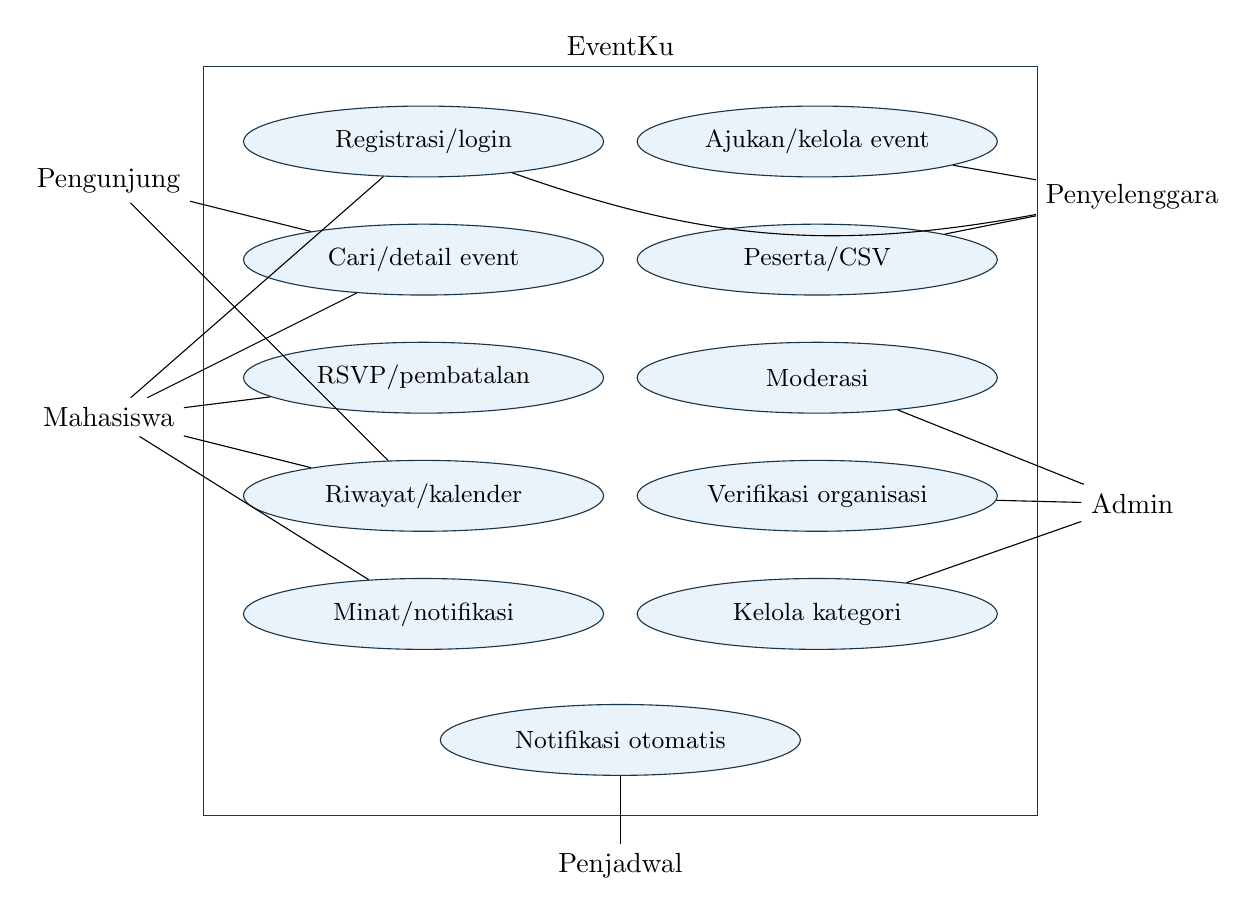
\begin{tikzpicture}
\node[uc] (u1) at (0,0) {Registrasi/login};\node[uc] (u2) at (0,-1.5) {Cari/detail event};\node[uc] (u3) at (0,-3) {RSVP/pembatalan};\node[uc] (u4) at (0,-4.5) {Riwayat/kalender};\node[uc] (u5) at (0,-6) {Minat/notifikasi};
\node[uc] (u6) at (5,0) {Ajukan/kelola event};\node[uc] (u7) at (5,-1.5) {Peserta/CSV};\node[uc] (u8) at (5,-3) {Moderasi};\node[uc] (u9) at (5,-4.5) {Verifikasi organisasi};\node[uc] (u10) at (5,-6) {Kelola kategori};\node[uc] (u11) at (2.5,-7.6) {Notifikasi otomatis};
\node[draw=navy,fit=(u1)(u6)(u11),inner sep=.5cm,label=above:EventKu] {};
\node (g) at (-4,-.5) {Pengunjung};\node (s) at (-4,-3.5) {Mahasiswa};\node (o) at (9,-.7) {Penyelenggara};\node (a) at (9,-4.6) {Admin};\node (p) at (2.5,-9.2) {Penjadwal};
\draw (g)--(u2);\draw (g)--(u4);\foreach \u in {u1,u2,u3,u4,u5}\draw (s)--(\u);
\draw (o)--(u6);\draw (o)--(u7);\draw (o) to[bend left=15] (u1);\foreach \u in {u8,u9,u10}\draw (a)--(\u);\draw (p)--(u11);
\end{tikzpicture}}\par\small Gambar 2. Diagram digambar ulang dalam LaTeX berdasarkan SRS versi 2; bukan ekspor Lucidchart.\end{center}
Pengunjung mengakses katalog publik; mahasiswa mengelola pendaftaran dan notifikasi sendiri. Penyelenggara mengelola event serta peserta dalam lingkup organisasi yang diizinkan. Admin menjalankan verifikasi/moderasi. Backend tetap memeriksa semua izin walaupun UI telah membatasi menu.
\page{Deskripsi Use Case: RSVP}
\tbl{p{3cm}Y}{Elemen & UC-05 -- Mendaftar event\\\midrule
Aktor & Mahasiswa.\\
Tujuan & Satu pendaftaran aktif pada kegiatan pilihan.\\
Prakondisi & Login; event Disetujui, belum berakhir, memiliki kursi tersedia.\\
Pemicu & Tombol RSVP pada detail event.\\
Alur utama & (1) UI mengirim ID event; (2) server mengambil identitas JWT; (3) periksa status/waktu; (4) transaksi memeriksa pendaftaran dan mereservasi kursi; (5) simpan/aktifkan pendaftaran; (6) commit; (7) kirim hasil; (8) publikasikan StudentRegistered.\\
Alternatif & Token tidak valid: login kembali. Penuh: tolak tanpa perubahan. Sudah aktif: tidak menambah kursi. Pernah dibatalkan: aktifkan ulang jika memenuhi syarat. Operasi gagal: rollback seluruh perubahan.\\
Pascakondisi & Satu pendaftaran aktif; penghitung bertambah satu dan tidak melebihi kuota.\\
Kebutuhan & FR-RSV-01,02,06; konfirmasi in-app FR-RSV-05 adalah Should.\\}
\subsection{Pembatalan}
Mahasiswa hanya membatalkan pendaftaran sendiri sebelum waktu mulai. Perubahan status dan pengembalian kursi berada dalam satu transaksi. Permintaan pembatalan ulang tidak mengurangi penghitung lagi. Riwayat tetap tersedia.
\subsection{Skenario Penerimaan}
\begin{enumerate}
\item Dua permintaan kursi terakhir: hanya satu berhasil.
\item Permintaan ulang pendaftaran aktif: tidak membuat rekaman/reservasi baru.
\item Gagal menyimpan sesudah reservasi: rollback mengembalikan penghitung.
\item Pembatalan lintas akun atau sesudah mulai: ditolak tanpa perubahan.
\end{enumerate}
Skenario di atas adalah rencana validasi, bukan hasil uji aktual.
\page{Deskripsi Use Case: Pengajuan dan Moderasi}
\tbl{p{2.6cm}Y}{Elemen & UC-10 -- Mengajukan event\\\midrule
Aktor/tujuan & Penyelenggara; meminta persetujuan publikasi.\\
Prakondisi & Login, organisasi terverifikasi, memiliki hak terhadap draft.\\
Alur utama & Isi judul, deskripsi, kategori, mulai/selesai, lokasi/tautan, poster dan kuota. Server memvalidasi. Simpan Draft lalu ajukan menjadi Menunggu Moderasi.\\
Alternatif & Data salah, akhir tidak sesudah mulai, organisasi belum terverifikasi, atau draft pihak lain: ditolak dengan alasan yang sesuai.\\
Pascakondisi & Masuk antrean admin, belum menjadi katalog publik.\\
Kebutuhan & FR-AUTH-05; FR-EVT-01--05.\\}
\vspace{.4cm}
\tbl{p{2.6cm}Y}{Elemen & UC-13 -- Moderasi event\\\midrule
Aktor/tujuan & Admin; memutuskan kelayakan publikasi.\\
Prakondisi & Login admin; event Menunggu Moderasi.\\
Alur utama & Buka antrean/detail. Setujui atau tolak dengan alasan. Server memeriksa transisi, menyimpan keputusan, commit, mempublikasikan EventModerated; persetujuan juga mempublikasikan EventApproved.\\
Alternatif & Alasan kosong: minta perbaikan. Status berubah: tolak transisi/muat ulang. Token atau peran salah: tolak akses.\\
Pascakondisi & Disetujui atau Ditolak; hasil in-app untuk penyelenggara. Persetujuan membuka katalog dan notifikasi minat.\\
Kebutuhan & FR-MOD-01--04; riwayat FR-MOD-06 adalah Should.\\}
Versi keputusan mencegah notifikasi moderasi berikutnya hilang karena deduplikasi terlalu umum. Edit penting setelah persetujuan memerlukan moderasi ulang jika fitur Should tersebut diimplementasikan.
\page{Arsitektur Sistem}
\subsection{Modular Monolith}
Satu backend Express.js memiliki empat modul. Pilihan ini mengurangi beban operasional tim kecil dan memungkinkan transaksi database bersama, sekaligus menjaga batas tanggung jawab. Frontend React/Tailwind berkomunikasi melalui HTTP/JSON.
\lucidfig{arsitektur_modular}{.48\textheight}{Gambar 3. Arsitektur modular EventKu (ekspor Lucidchart).}
\note{Database yang dipilih adalah PostgreSQL, sesuai konfirmasi Bambang dan README yang menggunakan Neon PostgreSQL. Rencana hosting tetap Vercel untuk frontend dan Render untuk backend. Pilihan tipe ID UUID/BIGINT masih perlu ditetapkan sebelum migrasi dibuat.}

\page{Rancangan Antarmuka Figma}
Rancangan UI dibuat Audrey pada Minggu 7 dan digunakan sebagai acuan visual awal. Sembilan tampilan yang tersedia mencakup Home, Login, Register, Dashboard Mahasiswa, Detail Event, Calendar, Kelola Event, Tambah Event dan Edit Event. Gambar diambil tanpa mengubah isi dari dokumen UI kelompok.
\subsection{Home dan Pencarian}
Home menampilkan navigasi, kata kunci, kategori dan kartu event mendatang. Tampilan ini mendukung alur pencarian dan pembukaan detail kegiatan (UC-03 dan UC-04).
\uifig{home}{.50\textheight}{Gambar UI-1. Home EventKu pada rancangan Figma.}
\href{https://www.figma.com/design/msefrhl4aO32NFpVU4MRlo/RPL-EventKu--UTS-}{Buka desain Figma}\quad\href{https://www.figma.com/proto/msefrhl4aO32NFpVU4MRlo/RPL-EventKu--UTS-?node-id=1-52}{Buka prototype Figma}.
\note{Mockup merupakan rancangan visual, bukan bukti implementasi atau seluruh kebutuhan SRS sudah tercakup. Hak akses dan status tetap mengikuti SRS versi 2.}
\clearpage\subsection{Detail Event dan RSVP}
Detail event menampilkan poster, jadwal, lokasi, penyelenggara, kuota, deskripsi dan tombol daftar. Alur ini mendukung UC-04 dan UC-05. Tombol Simpan Event pada mockup merupakan fitur bookmark berprioritas Could, sehingga bukan lingkup wajib MVP.
\uifig{detail_event}{.53\textheight}{Gambar UI-2. Detail event dan tombol pendaftaran pada Figma.}
\subsection{Cakupan dan Penyesuaian saat Implementasi}
Dashboard mahasiswa, kalender dan halaman pengelolaan tersedia pada lampiran. Label Admin/Campus dan Dipublikasikan pada mockup dipertahankan sebagai bukti desain awal. Implementasi memakai pembagian hak akses penyelenggara terverifikasi dan admin serta enam status yang ditentukan SRS. Form waktu mulai/selesai, moderasi, minat/notifikasi, dan tampilan mobile perlu dirinci mengikuti SRS tanpa menganggap semua sudah tergambar.
\page{Tanggung Jawab dan Aliran Data}
\tbl{p{3cm}Y}{Komponen & Tanggung jawab\\\midrule
View React & Form, hasil, loading/error dan navigasi; tidak menetapkan izin server.\\
Hooks/API client & Aksi UI, validasi awal, permintaan HTTP dan pembaruan data halaman.\\
Context & State sesi/peran/organisasi bersama; bukan pengganti aturan bisnis.\\
Controller & Request, aktor terverifikasi, pemanggilan service, HTTP/DTO.\\
Service/domain & Aturan bisnis, transisi status, kepemilikan dan transaksi.\\
Repository & SQL berparameter, filter, pagination, kontrak yang dapat diuji.\\
Facade publik & Akses lintas modul tanpa mengimpor repository privat.\\
EventBus / handler & Event setelah commit; pemilihan penerima notifikasi.\\}
\subsection{Aliran Pencarian}
View mengirim GET /api/v1/events. Controller dan service menormalisasi query serta menetapkan lingkup publik Disetujui. Repository menggunakan filter identik untuk count dan daftar, dengan urutan stabil. Controller mengirim JSON; UI menampilkan hasil atau keadaan kosong.
\subsection{Modularitas dan Kualitas}
Kontrak publik menjaga batas modul; pemisahan UI, bisnis dan SQL membantu pemeliharaan. Pagination, indeks dan backend stateless mendukung skalabilitas awal. Pada peningkatan pengguna sepuluh kali, ukur query pencarian, koneksi database, serta kontensi kuota sebelum memilih caching atau pemisahan layanan.
EventBus in-process sesuai tahap awal, tetapi kegagalan proses setelah commit dapat melewatkan notifikasi. Outbox, worker, retry dan handler idempoten dapat dipertimbangkan jika diperlukan keandalan pengiriman lebih tinggi.
\subsection{Kontrak API Awal}
Kelompok endpoint meliputi auth/register, auth/login, events, pengajuan/moderasi, registrations, notifications, organisasi dan kategori. Identitas diambil dari JWT, bukan ID aktor bebas dari request. Respons membedakan 401 autentikasi, 403 izin, 404 data hilang, 409 konflik kuota/status/duplikasi, serta 422 input tidak valid.
\page{Rancangan Modul dan Struktur Data}
\subsection{Auth}
\tbl{p{2.7cm}Y}{Aspek & Rancangan\\\midrule
Tujuan & Akun, autentikasi dan identitas aktor.\\
Input & Nama, email, kata sandi, peran publik; kredensial login.\\
Proses & Validasi, email unik, hash, simpan; login memverifikasi hash dan menghasilkan JWT.\\
Output & UserDTO tanpa hash; token memiliki masa berlaku.\\
Dependensi & UserRepository, hash provider, JwtProvider, status organisasi.\\
Struktur data & User, Organization, claims; email unik dan peran terbatas.\\}
Admin tidak dibuat melalui signup publik. Status verifikasi diperiksa server. Strategi penyimpanan token perlu ditetapkan dengan mempertimbangkan risiko XSS dan kebutuhan sesi.
\subsection{Event dan Pendaftaran}
\tbl{p{2.7cm}Y}{Aspek & Rancangan\\\midrule
Tujuan & Publikasi kegiatan dan pendaftaran berkuota konsisten.\\
Input & EventDTO, filter, keputusan admin, ID event/pendaftaran, aktor JWT.\\
Proses & Validasi status/waktu/organisasi; moderasi; reservasi dan penyimpanan RSVP atomik.\\
Output & EventDTO, EventPage, RegistrationDTO; event setelah commit.\\
Dependensi & EventRepository, RegistrationRepository, EventPublicApi, TransactionManager, EventBus.\\
Struktur data & Event, EventCategory, Registration; indeks, pasangan event--mahasiswa unik, penghitung kursi.\\}
\subsection{Notifikasi}
Handler menerima EventModerated, EventApproved dan StudentRegistered sesuai prioritas fitur. CategorySubscription dipakai untuk event baru sesuai minat. Pengingat H-1 menargetkan peserta terdaftar aktif sesuai SRS. Daftar/baca notifikasi hanya boleh untuk identitas JWT sendiri.
\page{Algoritma Pencarian dan RSVP}
\subsection{Pencarian dengan Filter Konsisten}
\begin{lstlisting}
searchPublicEvents(input):
  validate page >= 1 and 1 <= limit <= 20
  normalize keyword, category, organizer
  validate date OR [from, to); reject mixed inputs
  filter = status DISETUJUI
  combine supplied keyword/category/organizer with AND
  add start_time >= from AND start_time < to
  total = repository.count(filter)
  data = repository.find(filter,
         order by start_time ASC, event_id ASC,
         limit, offset = (page - 1) * limit)
  return {data, total, page}
\end{lstlisting}
Query memakai parameter. Count dan daftar memakai predikat identik. Tanggal tunggal berarti satu hari dalam zona waktu aplikasi; batas akhir eksklusif menghindari tumpang tindih periode. Nama konstanta implementasi mengikuti enum final.
\subsection{Pendaftaran Atomik}
\begin{lstlisting}
register(eventId, actor):
  require authenticated student
  transaction(tx):
    event = events.getEvent(eventId, tx)
    validate approved and not ended
    previous = registrations.find(eventId, actor.id, tx)
    if previous is active: reject duplicate
    if not events.reserveSeat(eventId, tx): reject full
    save or reactivate registration in tx
  after commit: publish StudentRegistered
  return registration DTO
\end{lstlisting}
Reservasi menggunakan pembaruan bersyarat atau penguncian untuk menjaga kuota. Constraint unik menjadi pengaman terhadap permintaan akun yang sama. Gagal menyimpan membatalkan reservasi melalui rollback. Pembatalan hanya melepas kursi saat status berubah aktif menjadi dibatalkan.
\page{Penerapan Design Pattern}
\subsection{Observer -- Behavioral Pattern}
Masalahnya adalah memberi notifikasi atas perubahan domain tanpa mengikat layanan EventService dan RegistrationService secara langsung ke layanan NotificationService. Publisher memakai EventBus sesudah commit. Subscriber didaftarkan pada startup dan menangani event yang sesuai.
\lucidfig{observer}{.44\textheight}{Gambar 4. Observer antara Event, Pendaftaran dan Notifikasi (ekspor Lucidchart).}
EventModerated memberi hasil kepada penyelenggara; EventApproved memberi pemberitahuan sesuai kategori minat. StudentRegistered memberi konfirmasi bila fitur Should dipilih. Deduplikasi menggunakan sumber/versi keputusan, penerima dan tipe; satu event dapat dimoderasi lebih dari sekali.
\clearpage\subsection{Repository -- Pola Akses Data}
Service bergantung pada kontrak repository; implementasi SQL menyediakan pencarian dan penyimpanan. Pemisahan ini memungkinkan test double dan menjaga aturan bisnis dari rincian query. Repository adalah pola akses data, bukan kategori GoF.
\lucidfig{repository}{.40\textheight}{Gambar 5. Repository Pattern pada modul Event (ekspor Lucidchart).}
\subsection{MVC}
View React menerima JSON dari controller HTTP. Service, domain, dan repository menjalankan tanggung jawab model backend. Hooks mengoordinasikan aksi UI; Context membagikan state dan tidak dianggap seluruh controller. Aturan bisnis dapat diuji tanpa merender halaman.
\page{Progres sampai Minggu 8 dan Perubahan Kebutuhan}
Evaluasi progres UTS dibatasi pada Minggu 1--8. Pekerjaan Minggu 9--16 merupakan rencana lanjutan menuju UAS dan tidak dinilai sebagai kekurangan pelaksanaan UTS.

\begingroup
\small
\setlength{\tabcolsep}{3pt}
\tbl{>{\raggedright\arraybackslash}p{.6cm}>{\raggedright\arraybackslash}p{1.8cm}>{\raggedright\arraybackslash}p{1.2cm}Y>{\raggedright\arraybackslash}p{1.65cm}>{\raggedright\arraybackslash}p{3cm}}{No. & Rencana & Target minggu & Realisasi / bukti & Status artefak & Catatan jadwal / kendala\\\midrule
1 & Inisiasi & 1 & Charter dan identitas/peran tersedia. & Tersedia & Waktu persetujuan formal belum dibuktikan.\\
2 & Analisis & 2--4 & SRS, kebutuhan, user story dan backlog tersedia. & Tersedia & Ketepatan waktu belum dapat dipastikan dari commit saja.\\
3 & Diagram alur & 5 & Use case, activity diagram dan ERD draft tersedia. & Tersedia & Artefak rancangan; bukan hasil uji aplikasi.\\
4 & Arsitektur & 6 & Modular, class diagram, ERD dan Lucidchart tersedia. & Tersedia & Bambang tidak melaporkan kendala pribadi.\\
5 & Pattern / UI / QA & 7 & Pattern, Figma dan 35 test case tersedia. & Tersedia; uji belum dijalankan & Audrey: penentuan alur UI. Alexa: sebagian tugas selesai terlambat.\\
6 & Konsolidasi & 8 & DOCX, tautan, laporan, PPT dan empat analisis individu tersedia. & Untuk review akhir & Verifikasi bukti Dustin ditindaklanjuti oleh pemiliknya.\\
}
\endgroup
Status tabel menunjukkan ketersediaan artefak UTS, bukan persentase penyelesaian aplikasi atau pernyataan bahwa semua pekerjaan selesai tepat waktu. Realisasi tanggal setiap tugas hanya dapat dinyatakan jika didukung catatan tugas atau konfirmasi pemilik; tanggal commit tidak dipakai sebagai pengganti tanggal selesai.
\subsection{Kendala Aktual sampai Minggu 8}
Pada konfirmasi awal, Bambang tidak melaporkan kendala proyek sampai Minggu 8. Dalam evaluasi individu yang kemudian dilampirkan, Audrey menjelaskan kendala menentukan alur penggunaan aplikasi, sedangkan Alexa menyatakan seluruh tugas individunya telah selesai, meskipun beberapa melewati waktu yang direncanakan. Alexa sempat mengalami kendala memahami penggunaan Jira pada Minggu 3, tetapi pekerjaan tersebut akhirnya diselesaikan. Alexa tidak menyimpulkan bahwa keterlambatan individunya menyebabkan seluruh proyek terlambat. Dustin melaporkan sebagian pekerjaannya terlambat atau tertunda akibat pengelolaan waktu dan beban kerja serta kesalahan pengerjaan; ia tidak menyatakan bagian pekerjaannya sepenuhnya sesuai jadwal. Penilaian jadwal tim perlu dibedakan dari ketepatan waktu individu dan dibandingkan dengan target serta bukti aktual. \cite{audreyind,dustinind,alexaind}
\subsection{Riwayat Artefak}
Riwayat lokal memuat activity diagram dan UI high-fidelity pada 6 Oktober 2026; penyelarasan rancangan dengan SRS serta tautan Lucidchart pada 7 Oktober. Tanggal commit membuktikan perubahan artefak, bukan waktu seluruh aktivitas atau persetujuan tugas. Pada pemeriksaan Jira tanggal 19 Oktober 2026, enam item UTS tercatat Done dengan tenggat 19 Oktober 2026. SCRUM-3 diperjelas sebagai wireframe/alur UI, SCRUM-5 sebagai desain Figma, dan SCRUM-4 sebagai Task QA mandiri. Status Done merujuk artefak UTS; eksekusi uji aplikasi tetap belum dijalankan. Pembaruan administrasi Jira tidak mengganti tanggal penyelesaian asli atau bukti individu. \cite{jira}
\subsection{Perubahan yang Mempengaruhi Desain}
SRS terbaru mencakup organisasi/verifikasi, waktu mulai--selesai, enam status, hasil moderasi untuk penyelenggara dan prioritas notifikasi. ERD, class diagram, API dan testcase perlu selaras. Figma tidak diubah sesuai keputusan pengguna; implementasi mengikuti SRS dan perlu merinci cakupan UI yang belum tersedia.
\subsection{Keputusan Rancangan dan Tindak Lanjut}
\tbl{>{\raggedright\arraybackslash}p{2.5cm}>{\raggedright\arraybackslash}p{2.6cm}Y}{Aspek & Status & Keputusan / tindak lanjut\\\midrule
Database & Ditetapkan & PostgreSQL digunakan sebagai acuan laporan dan rancangan.\\
Tipe ID fisik & Belum ditetapkan & Architect dan tim backend menetapkan UUID atau BIGINT sebelum migrasi Minggu 9; PK dan FK harus identik.\\
Durasi sprint & Usulan & PM/BA dan tim menyepakati pembagian Minggu 9--13. Usulan 2+2+1 minggu belum dinyatakan sebagai keputusan tim.\\
Cakupan UI & Desain UTS tersedia & Figma dipertahankan. Kebutuhan SRS yang belum memiliki layar dirinci sebelum implementasi.\\
Pengujian & Persiapan tersedia & 35 test case belum dijalankan; hasil aktual dicatat setelah aplikasi tersedia.\\}
Keputusan yang belum ditetapkan dicatat sebagai tindak lanjut setelah UTS. Status ini tidak mengubah jawaban analisis individu atau menyatakan implementasi telah selesai.
\page{Risiko dan Mitigasi}
\tbl{p{3.3cm}Yp{4.1cm}}{Risiko & Dampak & Mitigasi yang disarankan\\\midrule
Durasi sprint tidak konsisten & Target melampaui waktu. & Tetapkan durasi dalam lima minggu dan kapasitas.\\
Tipe ID belum ditetapkan & Migrasi dan tipe FK dapat tidak konsisten. & Tetapkan UUID/BIGINT dan zona waktu; gunakan PostgreSQL sesuai keputusan.\\
UI sebagian kebutuhan & Lingkup dianggap selesai dari tampilan. & Matriks SRS--UI--API--test; rincikan layar yang belum ada.\\
Persaingan kuota & Kursi terlampaui, data tidak konsisten. & Transaksi, conditional update/lock, constraint unik, uji konkurensi.\\
Akses lintas organisasi & Kebocoran atau perubahan data pihak lain. & Peran, verifikasi, ownership server pada setiap operasi.\\
Event notifikasi terlewat & Informasi gagal dikirim sesudah commit. & Idempotensi; dokumentasikan batas EventBus; pertimbangkan outbox.\\
Integrasi / perubahan file & Konflik merge, diagram tidak sinkron. & Pull/rebase sebelum push, review, pemilik file/PR.\\
Should/Could berlebihan & Must tidak selesai. & Prioritas alur end-to-end Must; review kapasitas.\\}
\subsection{Perbedaan Risiko dan Kendala Aktual}
Kendala individu yang dilaporkan adalah penentuan alur UI oleh Audrey, pengelolaan waktu dan beban kerja serta kesalahan pengerjaan oleh Dustin, serta ketepatan waktu tugas dan kesulitan awal memahami Jira oleh Alexa. Dalam revisinya, Alexa menegaskan bahwa seluruh tugas individunya telah selesai dan kendala Jira tersebut sudah diatasi. Matriks di atas berisi potensi risiko pengembangan berikutnya; daftar tersebut tidak menyatakan semua risiko telah terjadi. Kendala pribadi dan dampaknya pada jadwal keseluruhan perlu dinilai terpisah. \cite{audreyind,dustinind,alexaind}
PM/BA mengelola jadwal/prioritas; Architect menjaga kontrak; Backend/Frontend mengintegrasikan; QA/DevOps memverifikasi kualitas dan lingkungan. Review bersama diperlukan agar penanganan risiko tercatat dan dapat ditindaklanjuti.
\page{Rencana Setelah UTS}
\tbl{p{2.6cm}Yp{3.9cm}}{Periode usulan & Fokus & Bukti selesai\\\midrule
Minggu 9--10 & Setup DB/API/UI, Auth, organisasi/verifikasi, draft/pengajuan/moderasi. & Migrasi, integrasi, uji izin, demo.\\
Minggu 11--12 & Katalog/filter/detail, RSVP atomik, pembatalan, kalender. & Uji count/filter, konkurensi/duplikasi, demo.\\
Minggu 13 & Minat/notifikasi Must, dashboard/CSV, integrasi. & Uji penerima, CSV/ownership; review Must.\\
Minggu 14--16 & Sistem, UAT, performa, deployment, serah terima. & Hasil aktual, konfigurasi, dokumentasi pengguna.\\}
Pembagian ini usulan berdasarkan rentang kalender; perlu disepakati tim. Should/Could dipilih setelah Must stabil.
\subsection{Ketertelusuran Contoh}
\tbl{p{3cm}p{2.2cm}Y}{Kebutuhan & Use case & Verifikasi\\\midrule
FR-AUTH-04 & UC-02 & Token/peran salah dan akses lintas akun ditolak.\\
FR-MOD-02--04 & UC-13 & Alasan wajib; hasil sampai ke penyelenggara.\\
FR-SRC-02/03 & UC-03 & Filter dan count sesuai dataset.\\
FR-RSV-02/06 & UC-05 & Duplikasi dan permintaan kursi terakhir.\\
FR-NTF-02 & UC-09/17 & Penerima kategori sesuai, tidak duplikat.\\
FR-DSH-04 & UC-12 & CSV sesuai event dan izin.\\}
Setiap perubahan memperbarui ID/versi SRS, kontrak API, diagram, backlog dan testcase. Kemajuan dinilai dari fungsi yang dapat diperagakan dan bukti uji; bukan persentase tanpa dasar.
\page{Pengujian dan UAT: Ruang Lingkup dan Lingkungan}\label{sec:uat-env}
Bagian ini menambahkan hasil pengujian Minggu 10--14 pada laporan UTS. Acuan kebutuhan tetap SRS versi 2 dan backlog Minggu 9; ruang lingkup adalah kebutuhan Must (autentikasi, pengajuan dan moderasi event, katalog dan pencarian, RSVP, kalender, notifikasi minat, dashboard). Dua jenis bukti harus dibedakan: pengujian fungsional otomatis pada API yang sudah dijalankan (Bagian~\ref{sec:uat-base}--\ref{sec:uat-bug}) dan UAT bersama pengguna nyata (Bagian~\ref{sec:uat-user}) yang hasilnya masih harus diisi tim.
\note{Pengujian otomatis awal (commit \texttt{5edd1e0}) dijalankan dengan bantuan asisten AI pada sandbox Linux dengan database in-memory (pg-mem), lalu \textbf{dijalankan ulang di mesin lokal tim (Windows)} pada commit \texttt{dccaa91} setelah perbaikan BUG-01 dan BUG-02. Verifikasi tambahan pada commit \texttt{ce114e9} (sandbox AI) dan eksekusi ulang menyeluruh pada commit \texttt{0a69a27} di mesin lokal Windows (25 November 2026) menghasilkan status lulus 100\% untuk Jest (termasuk \texttt{uat-retest.test.js}), Vitest, dan build produksi; tangkapan layar terminal lokal dilampirkan pada Bagian~\ref{sec:uat-base}. Pengujian API tetap memakai \texttt{pg-mem} dan bukan situs produksi; hasilnya adalah bukti kondisi kode dan bukan pengganti UAT bersama pengguna nyata.}
\subsection{Lingkungan dan Metode}
\tbl{p{4cm}Y}{Aspek & Keterangan\\\midrule
Versi aplikasi & Branch \texttt{main}, pengujian awal commit \texttt{5edd1e0} (59/61 lulus), perbaikan pada commit \texttt{dccaa91} (61/61 lulus), dan verifikasi ulang lokal lengkap bersama \texttt{uat-retest.test.js} pada commit \texttt{0a69a27} di repositori alexabilxiz/UAS\_PROJEK\_RPL\_EventKu.\\
Tanggal pengujian & 24--25 November 2026.\\
Runtime & Node.js v22, npm 10 (mesin lokal Windows; uji awal sandbox memakai Node.js v22.23.5).\\
Database & PostgreSQL in-memory (pg-mem) dengan skema dari \texttt{backend/db}; \textbf{bukan} PostgreSQL produksi (Neon).\\
Lingkungan & Mesin lokal Windows untuk verifikasi ulang (Jest/Supertest, Vitest, dan Playwright Chromium).\\
Data uji & Satu admin, dua penyelenggara (dua organisasi terverifikasi) dan satu penyelenggara organisasi belum terverifikasi, dua mahasiswa UKWMS, satu mahasiswa non-UKWMS, dua kategori.\\
Metode & Skrip alur lengkap: registrasi, login, logout, pengajuan, moderasi, katalog, RSVP, pembatalan, ekspor peserta; ditambah uji negatif (peran salah, lintas organisasi, input berbahaya, pembatasan login) dan uji regresi browser Playwright.\\}
\section{Hasil Uji Otomatis Bawaan Repositori}\label{sec:uat-base}
\tbl{p{4.5cm}p{3cm}Y}{Pemeriksaan & Hasil & Keterangan\\\midrule
Backend (Jest) & 62 dari 62 lulus & Delapan berkas: api-security, auth, frontend-contract, seed, uat-flow, uat-extra, uat-rate, uat-retest (commit \texttt{0a69a27}).\\
Frontend (Vitest) & 73 dari 73 lulus & Tujuh berkas pengujian (termasuk uji unit \texttt{logout} di \texttt{authService} dan \texttt{AuthContext}).\\
Build produksi frontend & Berhasil & Bundel JavaScript sekitar 114,7 KB (gzip) melalui \texttt{vite build}.\\
Verifikasi ulang perbaikan (\texttt{uat-retest.test.js}) & 17 dari 17 lulus & Sudah ditambahkan ke \texttt{backend/tests} (commit \texttt{0a69a27}) dan diverifikasi ulang di mesin lokal; rincian pada Bagian~\ref{sec:uat-api}.\\
Frontend browser (Playwright) & 36 regresi + 4 demo E2E lulus & Dijalankan di Chromium lokal (\texttt{frontend/e2e} terhadap fixture kontrak API dan \texttt{frontend/demo-e2e} pada server demo lokal, termasuk viewport 320/360 piksel).\\
Integrasi penuh lokal (Vite + Express + PostgreSQL 18.1) & 6 dari 6 lulus (0 error JS) & Pengujian browser Chromium nyata terhadap backend Express asli dan \textbf{PostgreSQL 18.1 lokal} (termasuk \texttt{db:migrate}, \texttt{db:seed}, uji konkurensi nyata 8 RSVP paralel untuk 1 kursi: 201=1, 409=7, \texttt{reserved\_seats=1/1}, verifikasi browser BUG-01 \& BUG-02, unggah poster, moderasi, kalender 360 piksel, dan ekspor CSV).\\
Verifikasi situs produksi live (Cloudflare Workers + Neon) & 6 dari 6 lulus (0 error aplikasi) & Verifikasi langsung pada \url{https://uas-projek-rpl-eventku.yuhugelo4.workers.dev} (commit \texttt{0e8c3bf}, Version ID \texttt{862f7ed6}): TLS \emph{Let's Encrypt} valid, \texttt{/health} 200 (273 ms), \texttt{/api/v1/categories} (3 kategori) \& \texttt{/api/v1/events} (10 event) membaca Neon PostgreSQL asli, auth PBKDF2 + header \texttt{nosniff} + blokir CORS lintas origin (836 ms), serta Playwright Chromium live desktop 1440 px dan mobile 360 px tanpa overflow horizontal.\\}
Aplikasi telah berhasil di-deploy pada satu Cloudflare Worker terpadu (\url{https://uas-projek-rpl-eventku.yuhugelo4.workers.dev}) yang terhubung ke Neon PostgreSQL produksi; pengujian baca, keamanan header/CORS, dan rendering browser live lulus pada Bukti QA-04 dan QA-05, sedangkan uji tulis penuh oleh 3--5 penguji nyata akan dicatat pada Bagian~\ref{sec:uat-user}.

\par\begin{center}\begin{minipage}{\linewidth}\centering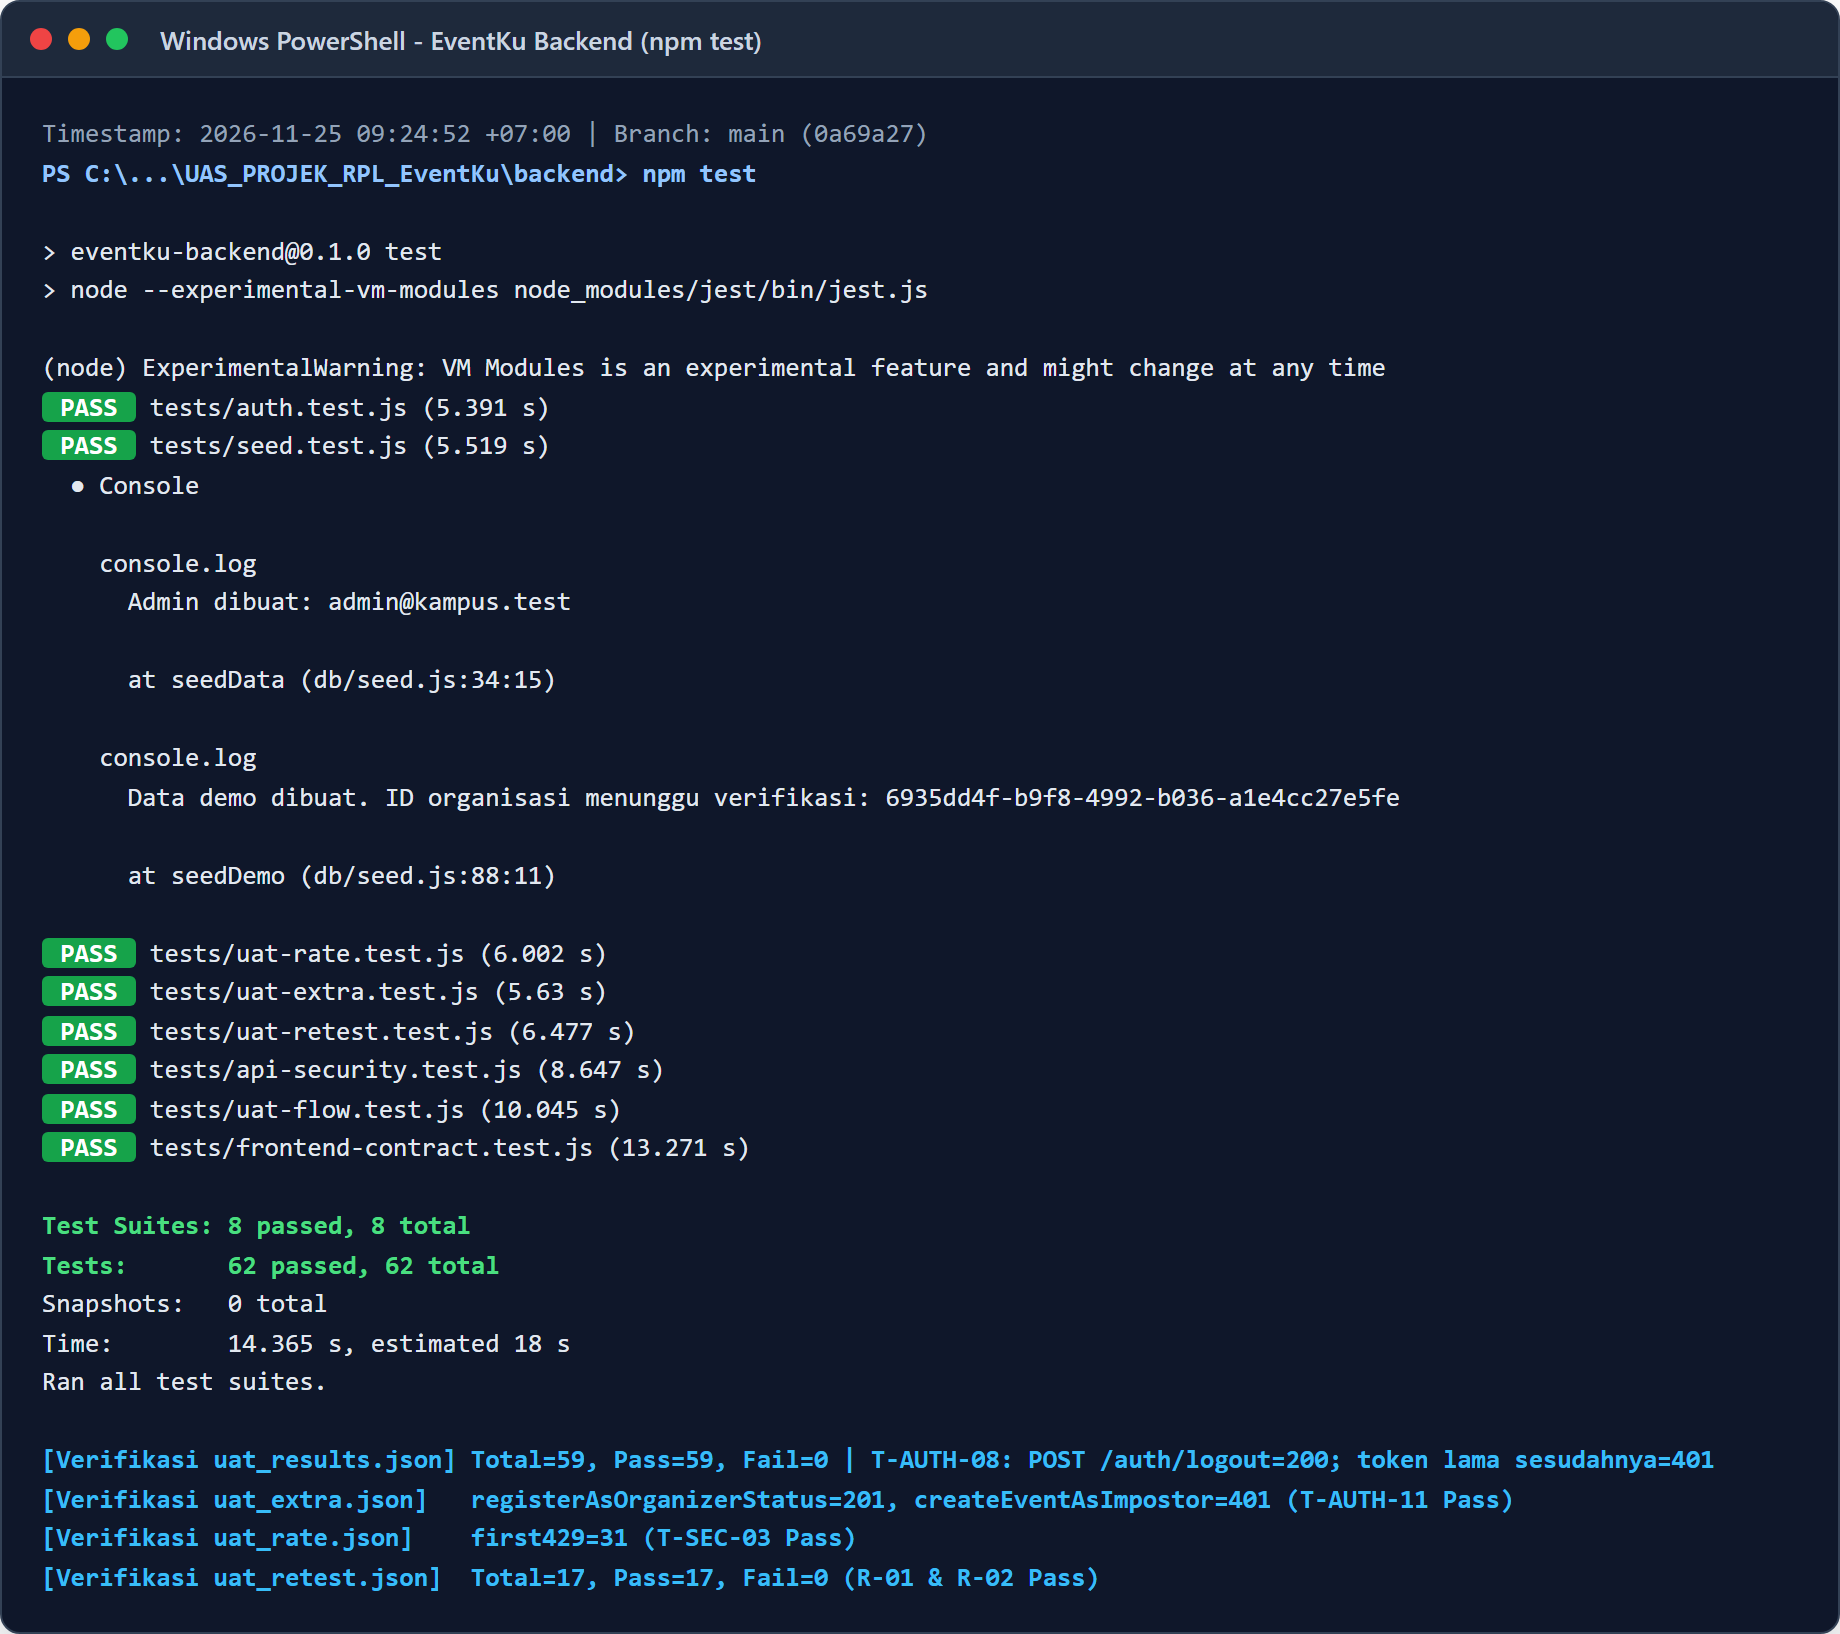
\includegraphics[width=\linewidth,height=.40\textheight,keepaspectratio]{figures/bukti_uji_backend_jest.png}\par\small Bukti QA-01. Hasil eksekusi ulang \texttt{npm test} backend (8/8 suite, 62/62 tes Jest + verifikasi UAT \& \texttt{uat-retest} 17/17 lulus pada \texttt{0a69a27}).\end{minipage}\end{center}\par
\par\begin{center}\begin{minipage}{\linewidth}\centering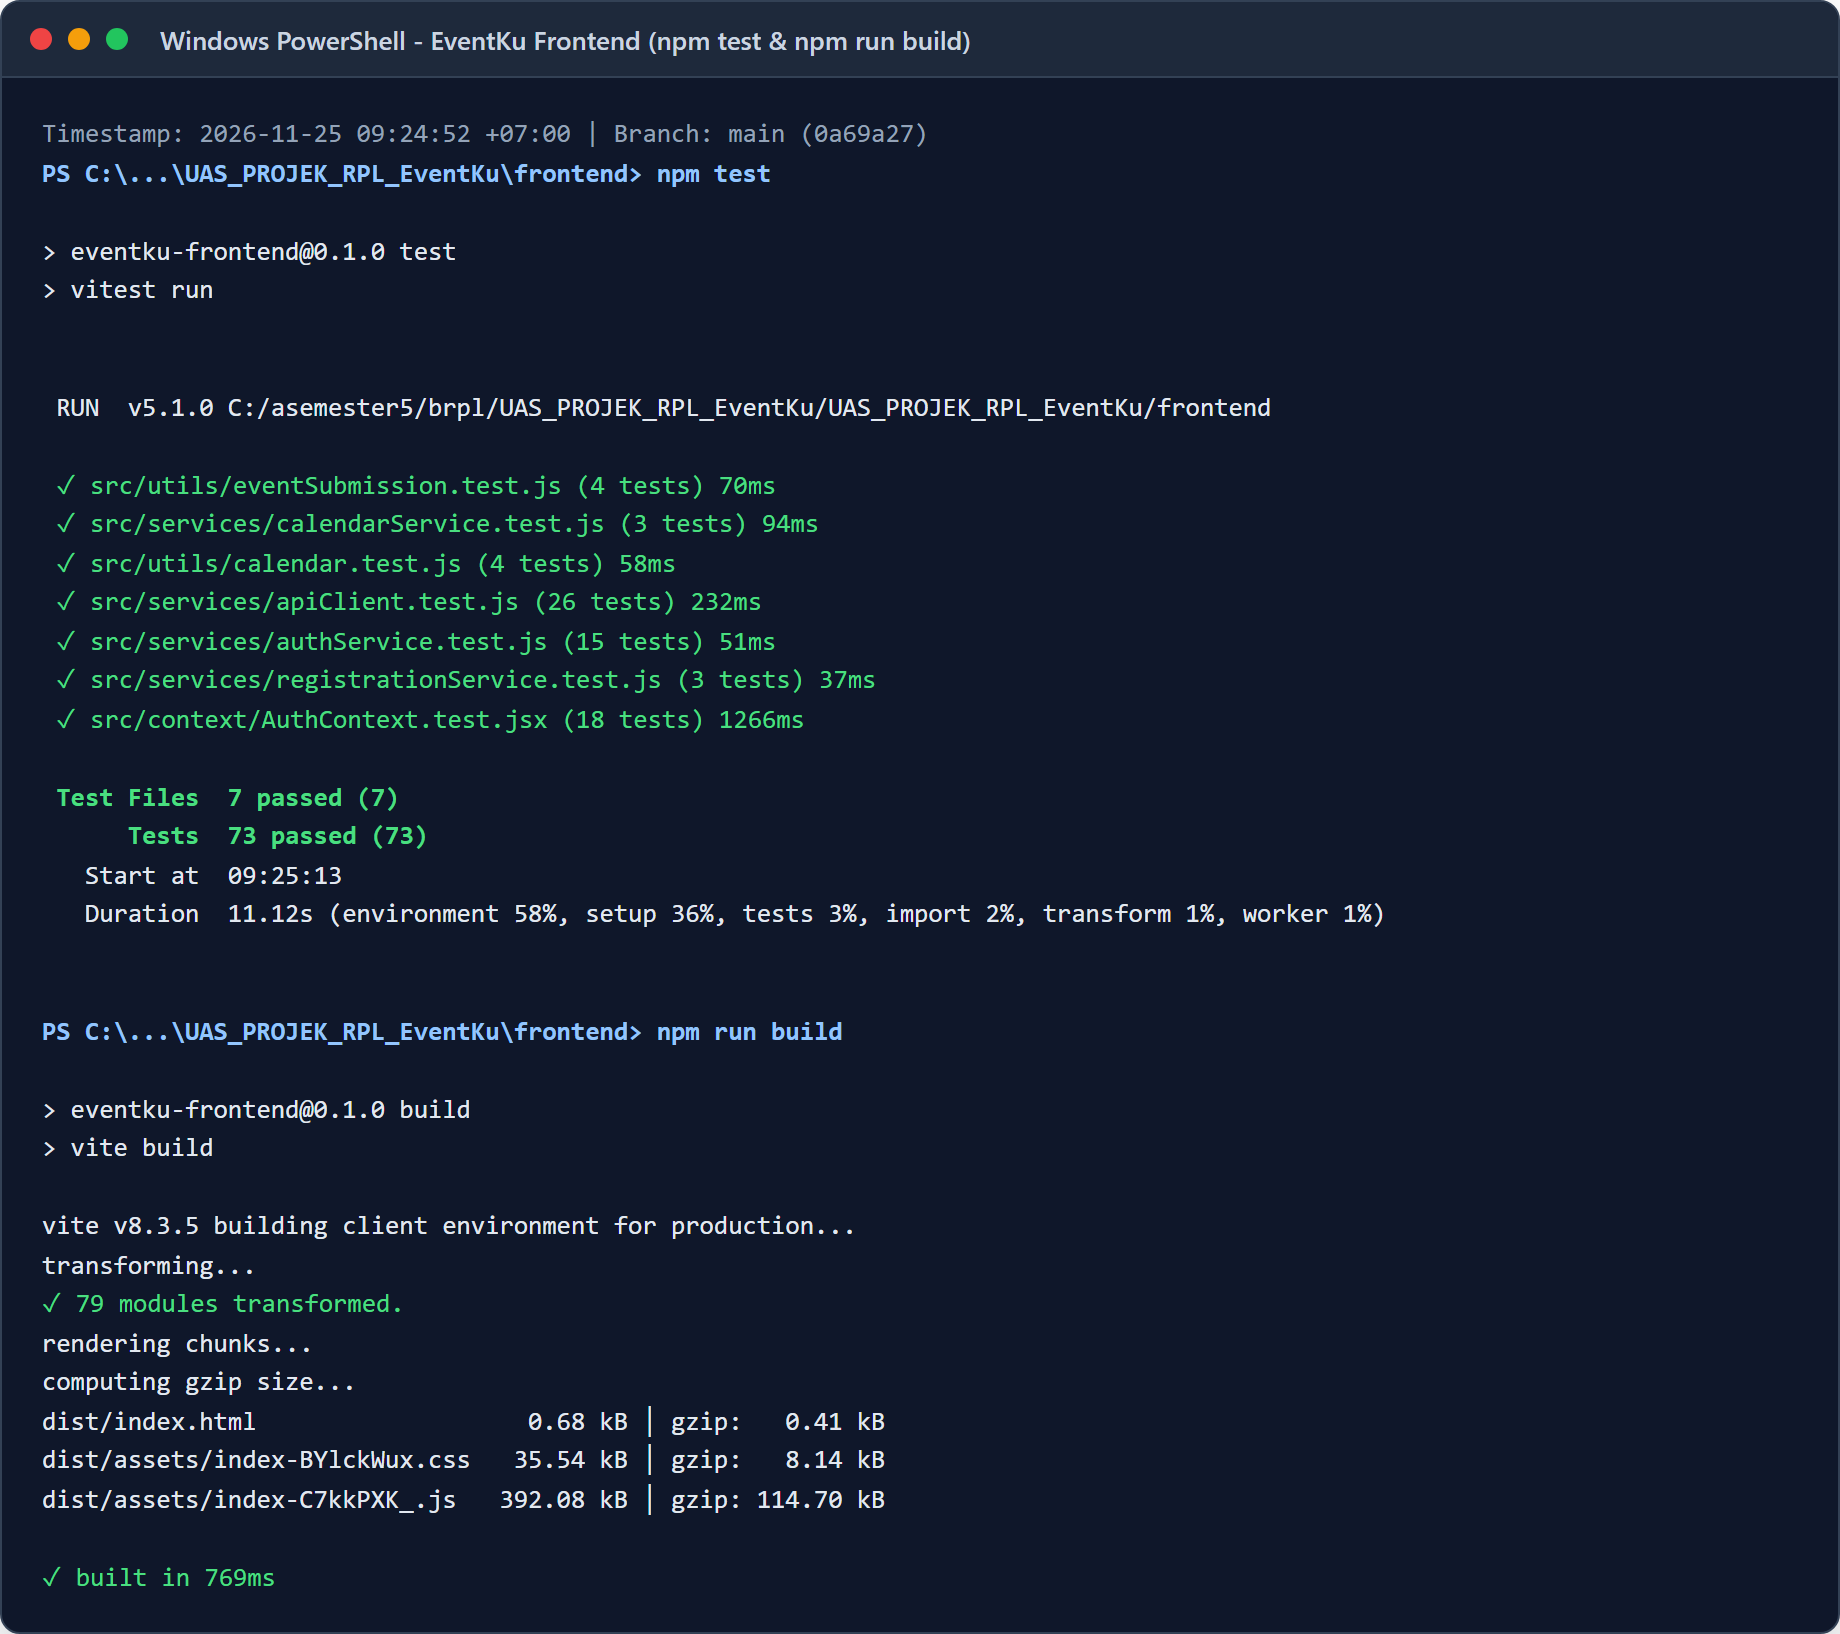
\includegraphics[width=\linewidth,height=.40\textheight,keepaspectratio]{figures/bukti_uji_frontend_vitest.png}\par\small Bukti QA-02. Hasil eksekusi ulang \texttt{npm test} (73/73 Vitest lulus) dan \texttt{npm run build} frontend pada \texttt{0a69a27}.\end{minipage}\end{center}\par
\par\begin{center}\begin{minipage}{\linewidth}\centering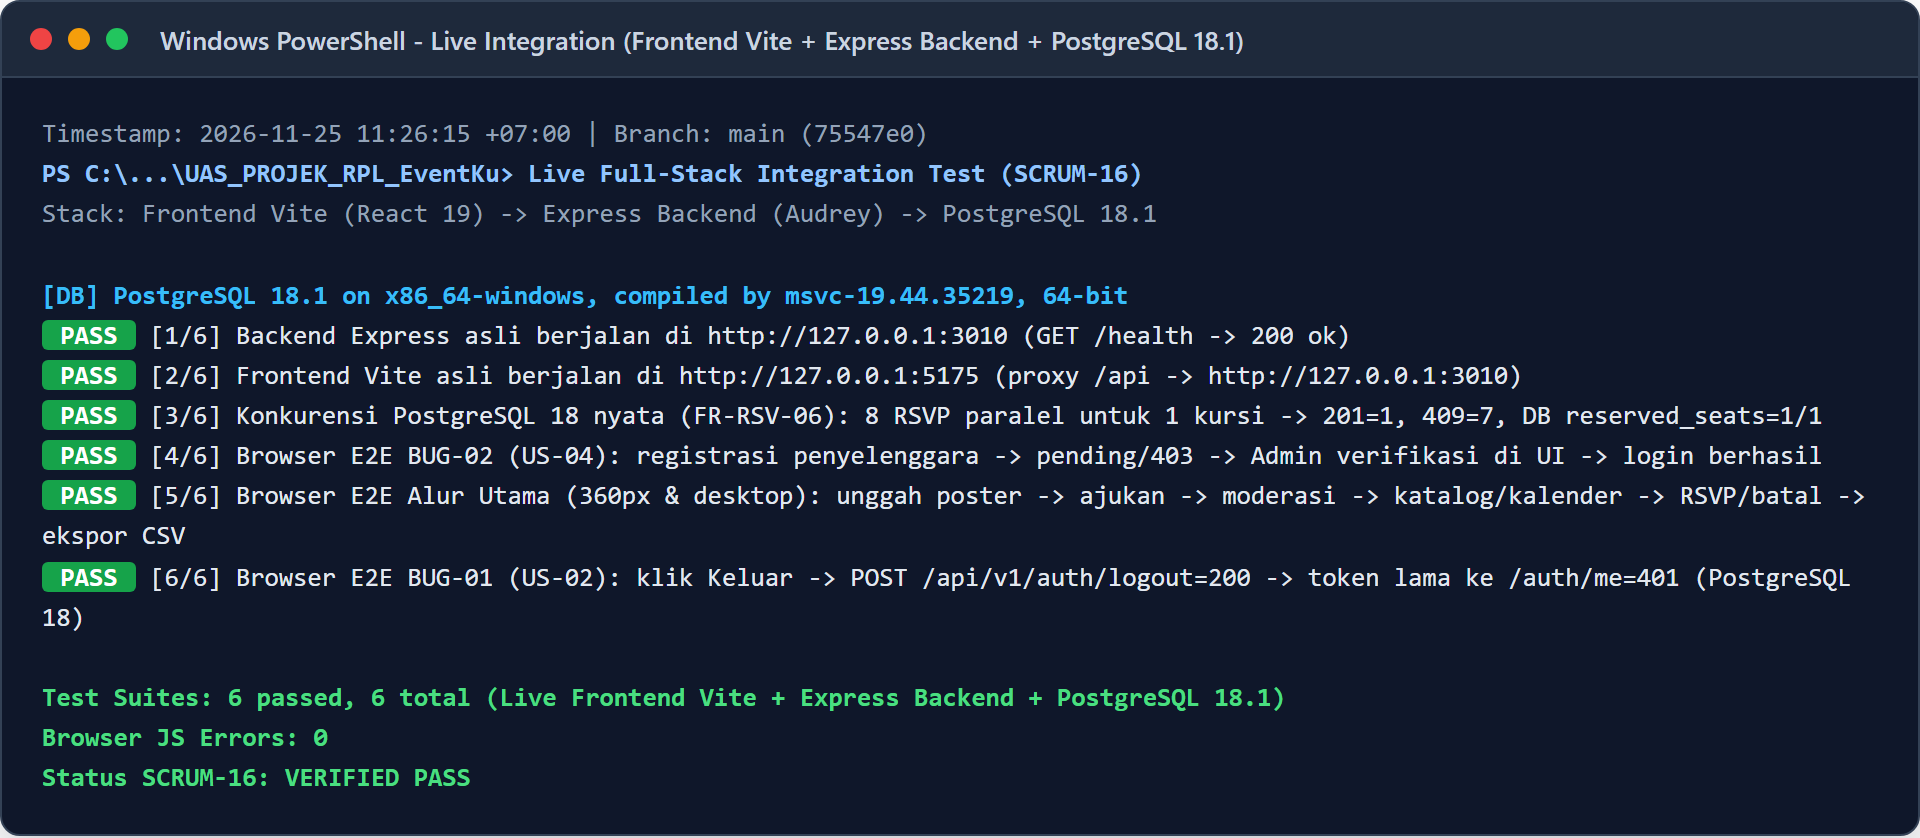
\includegraphics[width=\linewidth,height=.38\textheight,keepaspectratio]{figures/bukti_uji_integrasi_pg18.png}\par\small Bukti QA-03. Hasil uji integrasi penuh lokal Frontend Vite + Backend Express asli + PostgreSQL 18.1 (6/6 lulus, 0 error JS, verifikasi \texttt{SCRUM-16} dan konkurensi nyata FR-RSV-06).\end{minipage}\end{center}\par
\par\begin{center}\begin{minipage}{\linewidth}\centering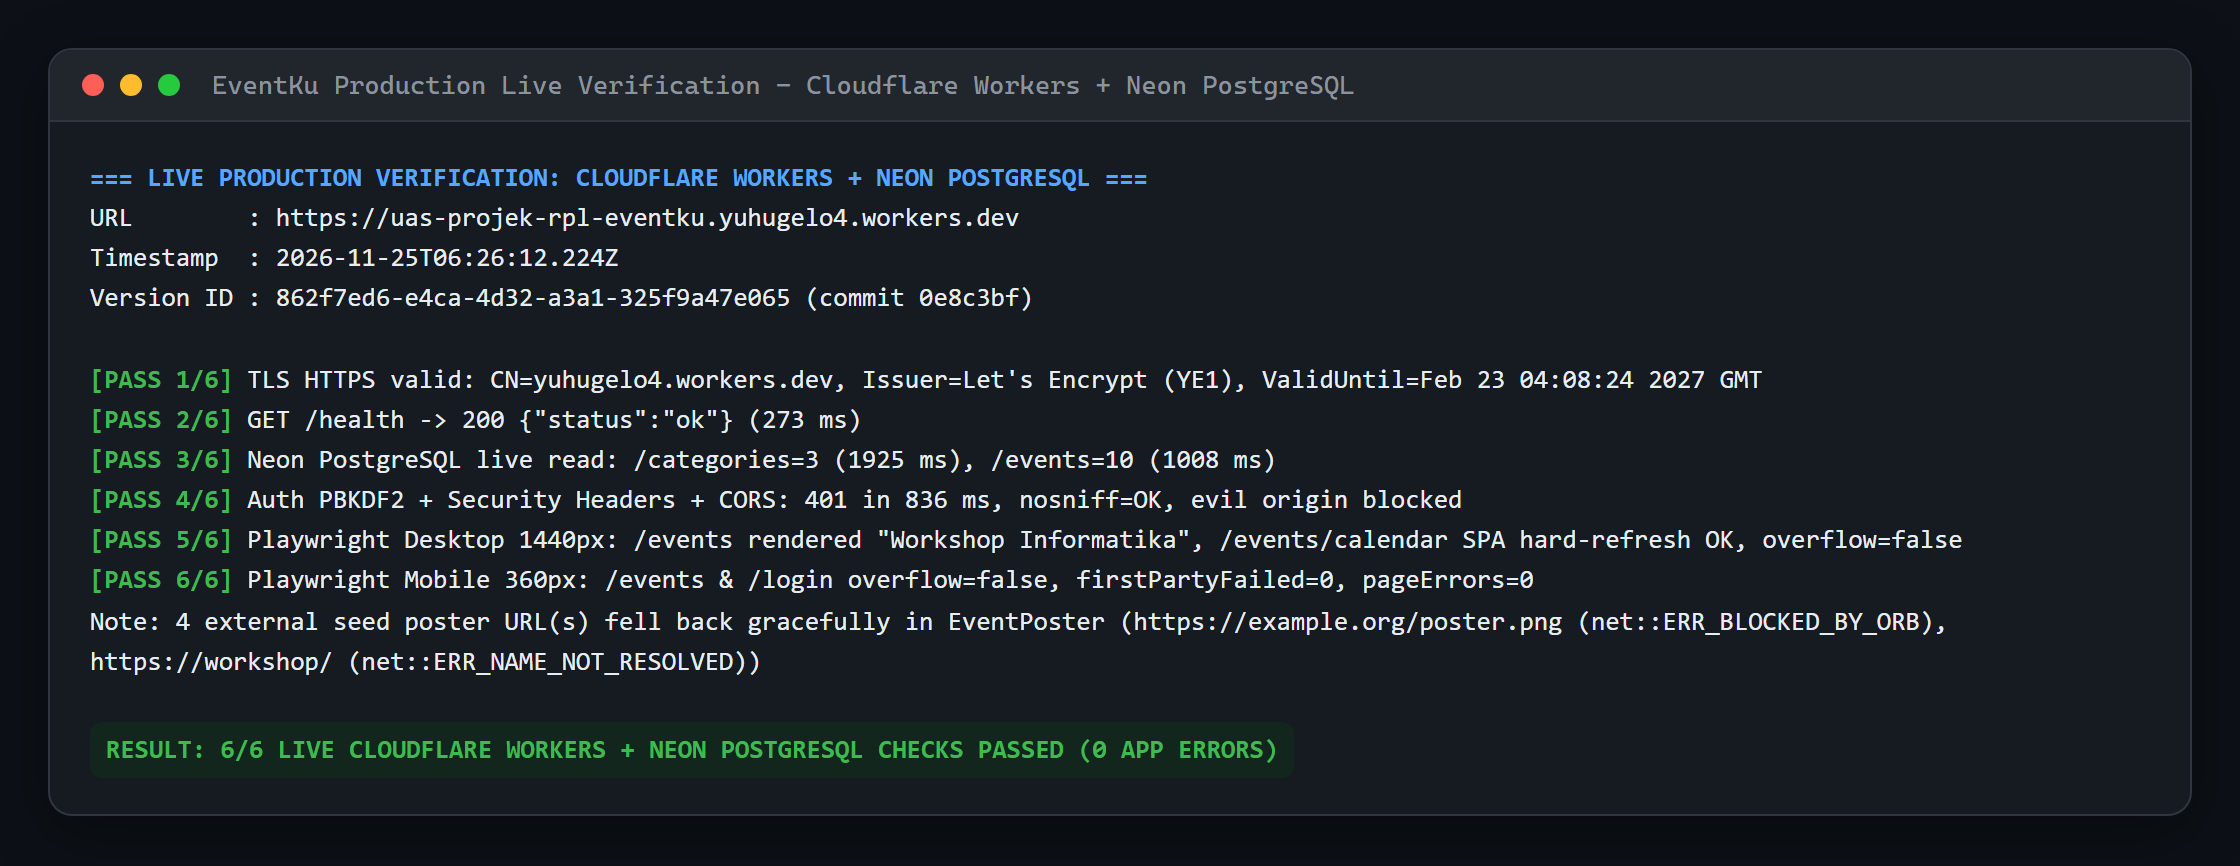
\includegraphics[width=\linewidth,height=.38\textheight,keepaspectratio]{figures/bukti_deploy_cloudflare_live.png}\par\small Bukti QA-04. Verifikasi situs produksi live \texttt{uas-projek-rpl-eventku.yuhugelo4.workers.dev} (Cloudflare Workers + Neon PostgreSQL, 6/6 lulus, commit \texttt{0e8c3bf}).\end{minipage}\end{center}\par
\par\begin{center}\begin{minipage}{\linewidth}\centering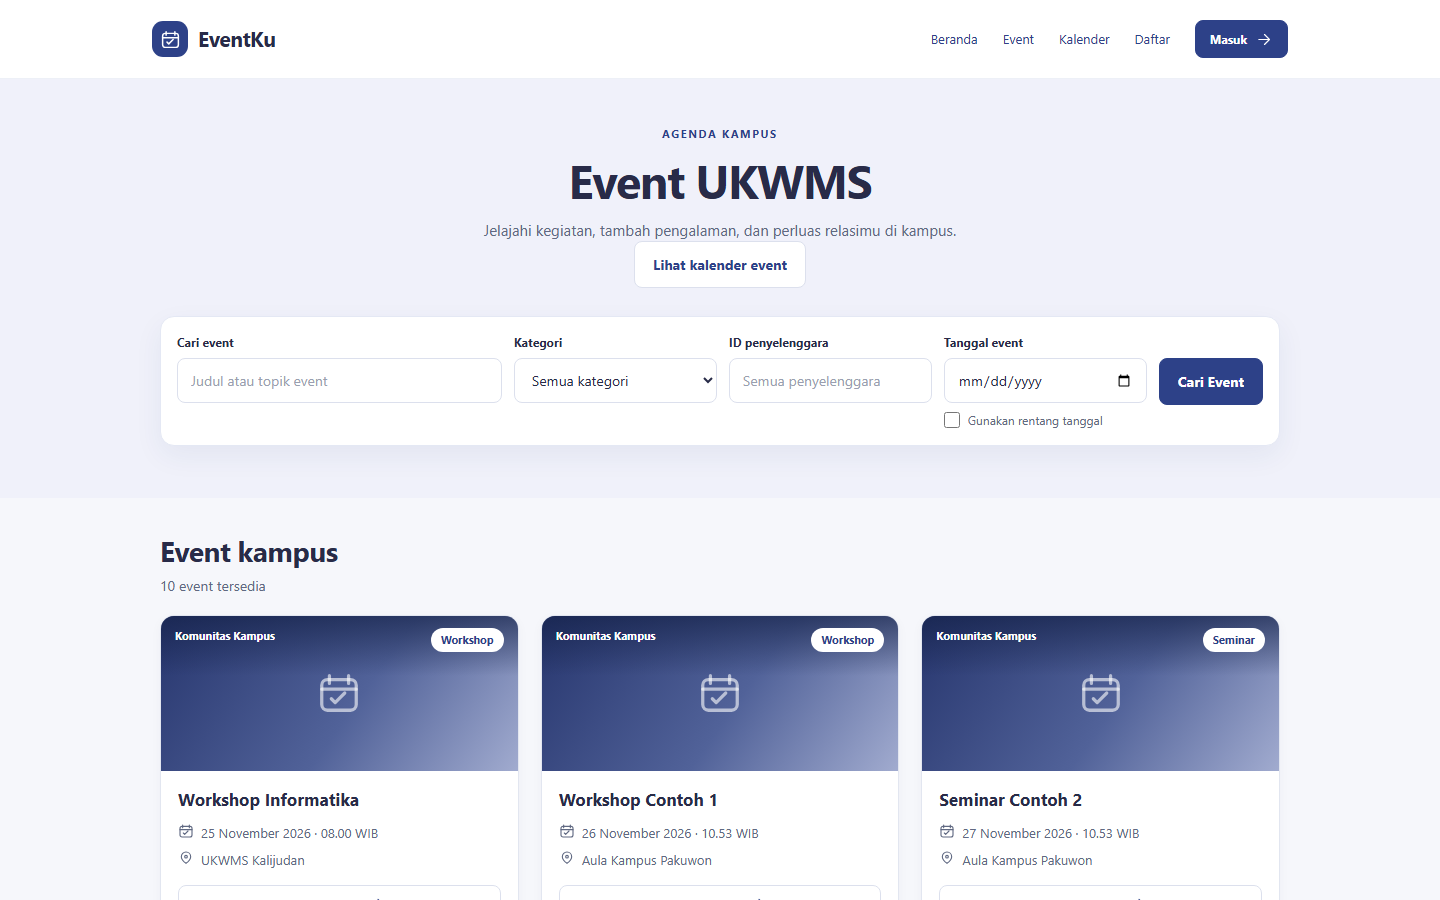
\includegraphics[width=\linewidth,height=.40\textheight,keepaspectratio]{figures/bukti_live_cloudflare_ui.png}\par\small Bukti QA-05. Tangkapan layar langsung katalog \texttt{/events} pada situs produksi Cloudflare Workers menampilkan 10 event aktif dari Neon PostgreSQL (desktop 1440 px, 0 overflow).\end{minipage}\end{center}\par
\section{Hasil Pengujian Fungsional API}\label{sec:uat-api}
Pada pengujian awal (commit \texttt{5edd1e0}), 59 dari 61 skenario lulus dan 2 gagal (97\%, yakni T-AUTH-08 dan T-AUTH-11). Setelah perbaikan BUG-01 dan BUG-02 pada commit \texttt{dccaa91} serta verifikasi ulang di mesin lokal, seluruh \textbf{61 dari 61 skenario lulus (100\%)}. Seluruh ID pada kolom Acuan ada di SRS versi 2; pemetaan ke isi kebutuhan diperiksa ulang pada 25 November 2026 dan 16 baris dikoreksi agar sesuai teks SRS (kelompok RSV, DSH, MOD, dan AUTH).
\subsection{Autentikasi dan hak akses}
{\footnotesize\setlength{\parskip}{0pt}\renewcommand{\arraystretch}{1.15}
\begin{longtable}{p{1.8cm}p{1.9cm}p{4.0cm}p{2.4cm}p{3.4cm}p{1.2cm}}
\toprule ID & Acuan & Skenario & Harapan & Hasil aktual & Status\\\midrule\endhead
\mbox{T-AUTH-01} & FR-AUTH-01 & Registrasi mahasiswa dengan data valid & 201 & 201 & \textbf{Lulus}\\
\midrule
\mbox{T-AUTH-02} & FR-AUTH-01 & Registrasi dengan email duplikat ditolak & 409 & 409 & \textbf{Lulus}\\
\midrule
\mbox{T-AUTH-03} & FR-AUTH-01 & Kata sandi \textless{} 8 karakter ditolak & 4xx & 422 & \textbf{Lulus}\\
\midrule
\mbox{T-AUTH-04} & FR-AUTH-01 & Registrasi publik dengan peran admin ditolak & 4xx & 422 & \textbf{Lulus}\\
\midrule
\mbox{T-AUTH-05} & FR-AUTH-03 & Login valid mengembalikan token & 200 + accessToken & 200 token=true & \textbf{Lulus}\\
\midrule
\mbox{T-AUTH-06} & FR-AUTH-03 & Login dengan kata sandi salah ditolak & 401 & 401 & \textbf{Lulus}\\
\midrule
\mbox{T-AUTH-07} & FR-AUTH-03 & Endpoint /me dengan token valid & 200 & 200 & \textbf{Lulus}\\
\midrule
\mbox{T-AUTH-08} & US-02 / FR-AUTH-03 & Logout menghapus sesi di server (token lama harus ditolak) & Token lama 401 setelah logout & Awal: 404/200; pasca-fix (\texttt{dccaa91}): POST /auth/logout=200; token lama=401 & \textbf{Lulus}\\
\midrule
\mbox{T-AUTH-09} & NFR-SEC-02 & Token JWT yang dimanipulasi ditolak & 401 & 401 & \textbf{Lulus}\\
\midrule
\mbox{T-AUTH-10} & NFR-SEC-03 & Akses tanpa token ditolak & 401 & 401 & \textbf{Lulus}\\
\midrule
\mbox{T-AUTH-11} & US-04 / FR-AUTH-05 & Akun penyelenggara baru tidak otomatis memperoleh hak atas organisasi terverifikasi sebelum diverifikasi admin & Akun menunggu verifikasi / pembuatan event ditolak & Awal: 201 aktif; pasca-fix (\texttt{dccaa91}): register=201 (\texttt{pending}); login=403; event/list=401 & \textbf{Lulus}\\
\midrule
\mbox{T-RBAC-01} & FR-AUTH-04 & Mahasiswa tidak boleh membuat event & 403 & 403 & \textbf{Lulus}\\
\midrule
\mbox{T-RBAC-02} & FR-AUTH-04 & Penyelenggara tidak boleh mengakses endpoint admin & 403 & 403 & \textbf{Lulus}\\
\midrule
\mbox{T-RBAC-03} & FR-AUTH-04 & Penyelenggara tidak boleh RSVP & 403 & 403 & \textbf{Lulus}\\
\midrule
\mbox{T-RBAC-04} & FR-AUTH-04 & Mahasiswa tidak boleh membuka dashboard penyelenggara & 403 & 403 & \textbf{Lulus}\\
\midrule
\mbox{T-RBAC-05} & FR-AUTH-04 & Penyelenggara tidak boleh memoderasi event & 403 & 403 & \textbf{Lulus}\\
\midrule
\mbox{T-SEC-03} & NFR-SEC-05 & Pembatasan percobaan login (rate limit) & 429 setelah batas percobaan & Permintaan ke-31 pada jendela 15 menit mendapat 429 & \textbf{Lulus}\\
\midrule
\bottomrule
\end{longtable}}
\subsection{Pengajuan event dan moderasi}
{\footnotesize\setlength{\parskip}{0pt}\renewcommand{\arraystretch}{1.15}
\begin{longtable}{p{1.8cm}p{1.9cm}p{4.0cm}p{2.4cm}p{3.4cm}p{1.2cm}}
\toprule ID & Acuan & Skenario & Harapan & Hasil aktual & Status\\\midrule\endhead
\mbox{T-EVT-01} & FR-AUTH-05 & Organisasi belum terverifikasi tidak boleh mengajukan event & 403 & 403 & \textbf{Lulus}\\
\midrule
\mbox{T-EVT-02} & FR-EVT-02 & Event tanpa judul ditolak & 4xx & 422 & \textbf{Lulus}\\
\midrule
\mbox{T-EVT-03} & FR-EVT-02 & Waktu selesai sebelum mulai ditolak & 4xx & 422 & \textbf{Lulus}\\
\midrule
\mbox{T-EVT-04} & FR-EVT-02 & Waktu mulai di masa lalu ditolak & 4xx & 422 & \textbf{Lulus}\\
\midrule
\mbox{T-EVT-05} & FR-EVT-02 & Kuota 0 ditolak & 4xx & 422 & \textbf{Lulus}\\
\midrule
\mbox{T-EVT-06} & FR-EVT-01 & Membuat draft event valid & 201 draft & 201 draft & \textbf{Lulus}\\
\midrule
\mbox{T-EVT-07} & FR-MOD-03 & Draft tidak tampil di katalog publik & 0 hasil & 0 & \textbf{Lulus}\\
\midrule
\mbox{T-EVT-08} & NFR-SEC-03 & Penyelenggara organisasi lain tidak boleh mengajukan draft ini & 404 & 404 & \textbf{Lulus}\\
\midrule
\mbox{T-EVT-09} & FR-EVT-03 & Ajukan draft -\textgreater{} menunggu moderasi & 200 menunggu\_moderasi & 200 menunggu\_moderasi & \textbf{Lulus}\\
\midrule
\mbox{T-EVT-10} & FR-EVT-03 & Pengajuan ganda ditolak & 409 & 409 & \textbf{Lulus}\\
\midrule
\mbox{T-EVT-11} & FR-MOD-03 & Event menunggu moderasi belum tampil publik & 0 hasil & 0 & \textbf{Lulus}\\
\midrule
\mbox{T-MOD-01} & FR-MOD-01 & Admin melihat antrean moderasi & total \textgreater{}= 1 & 1 & \textbf{Lulus}\\
\midrule
\mbox{T-MOD-02} & FR-MOD-02 & Penolakan tanpa alasan ditolak & 4xx & 422 & \textbf{Lulus}\\
\midrule
\mbox{T-MOD-03} & FR-MOD-02 & Admin menyetujui event & 200 disetujui & 200 disetujui & \textbf{Lulus}\\
\midrule
\mbox{T-MOD-04} & FR-MOD-02 & Moderasi ulang event yang sudah diputuskan ditolak & 409 & 409 & \textbf{Lulus}\\
\midrule
\mbox{T-MOD-05} & FR-MOD-04 & Penyelenggara menerima notifikasi hasil moderasi & Notifikasi diterima & Notifikasi status disetujui diterima & \textbf{Lulus}\\
\midrule
\mbox{T-MOD-06} & FR-MOD-06 & Riwayat moderasi tercatat & total \textgreater{}= 1 & 1 & \textbf{Lulus}\\
\midrule
\mbox{T-NTF-01} & FR-NTF-02 & Mahasiswa berminat kategori tersebut menerima notifikasi event baru & ada tipe event\_baru & ["event\_baru"] & \textbf{Lulus}\\
\midrule
\mbox{T-NTF-02} & FR-NTF-02 & Mahasiswa kategori lain TIDAK menerima notifikasi & tidak ada event\_baru & [] & \textbf{Lulus}\\
\midrule
\bottomrule
\end{longtable}}
\subsection{Katalog, pencarian, dan keamanan input}
{\footnotesize\setlength{\parskip}{0pt}\renewcommand{\arraystretch}{1.15}
\begin{longtable}{p{1.8cm}p{1.9cm}p{4.0cm}p{2.4cm}p{3.4cm}p{1.2cm}}
\toprule ID & Acuan & Skenario & Harapan & Hasil aktual & Status\\\midrule\endhead
\mbox{T-SEC-01} & NFR-SEC-04 & Input SQL injection pada pencarian tidak merusak data & 200 \& data utuh & 200, total=1 & \textbf{Lulus}\\
\midrule
\mbox{T-SEC-02} & NFR-SEC-04 & Judul berisi \textless{}script\textgreater{} tidak dieksekusi (API mengembalikan teks apa adanya; escape dilakukan React) & teks tersimpan sebagai string & Judul tersimpan sebagai teks biasa & \textbf{Lulus}\\
\midrule
\mbox{T-SRC-01} & FR-SRC-01 & Daftar event publik menampilkan event disetujui & total \textgreater{}= 1 & 1 & \textbf{Lulus}\\
\midrule
\mbox{T-SRC-02} & FR-SRC-02 & Pencarian kata kunci tidak sensitif huruf besar-kecil & total \textgreater{}= 1 & 1 & \textbf{Lulus}\\
\midrule
\mbox{T-SRC-03} & FR-SRC-02 & Pencarian tanpa hasil mengembalikan daftar kosong & 0 & 0 & \textbf{Lulus}\\
\midrule
\mbox{T-SRC-04} & FR-SRC-03 & Filter kategori sesuai data & cat=1, cat2=0 & cat=1, cat2=0 & \textbf{Lulus}\\
\midrule
\mbox{T-SRC-05} & FR-SRC-03 & Filter tanggal tidak valid ditolak & 4xx & 422 & \textbf{Lulus}\\
\midrule
\mbox{T-SRC-06} & FR-SRC-04 & ID event tidak valid -\textgreater{} 404 & 404 & 404 & \textbf{Lulus}\\
\midrule
\bottomrule
\end{longtable}}
\subsection{RSVP dan pembatalan}
{\footnotesize\setlength{\parskip}{0pt}\renewcommand{\arraystretch}{1.15}
\begin{longtable}{p{1.8cm}p{1.9cm}p{4.0cm}p{2.4cm}p{3.4cm}p{1.2cm}}
\toprule ID & Acuan & Skenario & Harapan & Hasil aktual & Status\\\midrule\endhead
\mbox{T-RSV-01} & FR-RSV-01 & Mahasiswa non-UKWMS tidak boleh RSVP & 403 & 403 & \textbf{Lulus}\\
\midrule
\mbox{T-RSV-02} & FR-RSV-06 & Dua permintaan untuk kursi terakhir: hanya satu berhasil & [201,409] & [201,409] & \textbf{Lulus}\\
\midrule
\mbox{T-RSV-03} & FR-RSV-02 & RSVP ganda pada event yang sama ditolak & 409 & 409 & \textbf{Lulus}\\
\midrule
\mbox{T-RSV-04} & NFR-SEC-03 & Pembatalan pendaftaran milik akun lain ditolak & 404 & 404 & \textbf{Lulus}\\
\midrule
\mbox{T-RSV-05} & FR-RSV-04 & Riwayat pendaftaran menampilkan event yang didaftari & total \textgreater{}= 1 & 1 & \textbf{Lulus}\\
\midrule
\mbox{T-RSV-06} & FR-RSV-03 & Pembatalan oleh pemilik sebelum event dimulai & 200 & 200 & \textbf{Lulus}\\
\midrule
\mbox{T-RSV-07} & FR-RSV-03 & Pembatalan ulang ditolak (kursi tidak dikembalikan dua kali) & 409 & 409 & \textbf{Lulus}\\
\midrule
\mbox{T-RSV-08} & FR-RSV-03 & Setelah pembatalan, kursi bisa dipakai pendaftar lain & 201 & 201 & \textbf{Lulus}\\
\midrule
\mbox{T-RSV-09} & FR-RSV-06 & Penghitung kursi konsisten (0 \textless{}= reserved \textless{}= quota) & reserved=1, quota=1 & \{"reserved\_seats":1,"quota":1\} & \textbf{Lulus}\\
\midrule
\mbox{T-RSV-10} & FR-RSV-01 & RSVP ke event yang tidak ada -\textgreater{} 404 & 404 & 404 & \textbf{Lulus}\\
\midrule
\bottomrule
\end{longtable}}
\subsection{Dashboard penyelenggara dan admin}
{\footnotesize\setlength{\parskip}{0pt}\renewcommand{\arraystretch}{1.15}
\begin{longtable}{p{1.8cm}p{1.9cm}p{4.0cm}p{2.4cm}p{3.4cm}p{1.2cm}}
\toprule ID & Acuan & Skenario & Harapan & Hasil aktual & Status\\\midrule\endhead
\mbox{T-ADM-01} & FR-ADM-04 & Statistik admin dapat diakses & 200 & 200 & \textbf{Lulus}\\
\midrule
\mbox{T-ADM-02} & FR-ADM-01 & Kategori duplikat ditolak & 409 & 409 & \textbf{Lulus}\\
\midrule
\mbox{T-ADM-03} & FR-ADM-02 & Admin membuat \& memverifikasi organisasi & 200 verified & 200 verified & \textbf{Lulus}\\
\midrule
\mbox{T-DSH-01} & FR-DSH-02 & Penyelenggara melihat daftar peserta eventnya & total=1 & 1 & \textbf{Lulus}\\
\midrule
\mbox{T-DSH-02} & NFR-SEC-03 & Penyelenggara organisasi lain tidak boleh melihat peserta & 404 & 404 & \textbf{Lulus}\\
\midrule
\mbox{T-DSH-03} & FR-DSH-04 & Ekspor CSV peserta & Header + 1 baris data & Header + 1 baris data & \textbf{Lulus}\\
\midrule
\mbox{T-DSH-04} & FR-DSH-03 & Statistik penyelenggara dapat diakses & 200 & 200 & \textbf{Lulus}\\
\midrule
\bottomrule
\end{longtable}}

\subsection{Verifikasi Ulang Perbaikan BUG-01 dan BUG-02}
Pengecekan tambahan pada commit \texttt{ce114e9}: 17 dari 17 lulus. Skenario R-02-xx menguji alur persetujuan akun penyelenggara (termasuk upaya mengubah status lewat isian registrasi), dan R-01-xx menguji logout (termasuk sesi paralel pada dua perangkat).
{\footnotesize\setlength{\parskip}{0pt}\renewcommand{\arraystretch}{1.15}
\begin{longtable}{p{1.8cm}p{1.9cm}p{4.0cm}p{2.4cm}p{3.4cm}p{1.2cm}}
\toprule ID & Acuan & Skenario & Harapan & Hasil aktual & Status\\\midrule\endhead
\mbox{R-02-01} & US-04 & Registrasi penyelenggara menghasilkan akun berstatus menunggu & 201 pending & 201 pending & \textbf{Lulus}\\
\midrule
\mbox{R-02-02} & US-04 & Akun menunggu tidak bisa login & 403 & 403 Akun penyelenggara menunggu verifikasi admin. & \textbf{Lulus}\\
\midrule
\mbox{R-02-03} & US-04 & Mass assignment: field status=active pada registrasi diabaikan & pending & pending & \textbf{Lulus}\\
\midrule
\mbox{R-02-04} & US-04 & Akun dengan status dipaksa active tetap tidak bisa login & 403 & 403 & \textbf{Lulus}\\
\midrule
\mbox{R-02-05} & FR-AUTH-01 & Registrasi mahasiswa tetap langsung aktif & 201 active & 201 active & \textbf{Lulus}\\
\midrule
\mbox{R-02-06} & FR-ADM-02 & Admin dapat menemukan akun penyelenggara yang menunggu & akun p1 terdaftar & ditemukan & \textbf{Lulus}\\
\midrule
\mbox{R-02-07} & FR-AUTH-04 & Penyelenggara tidak boleh menyetujui akun penyelenggara lain & 403 & 403 & \textbf{Lulus}\\
\midrule
\mbox{R-02-08} & FR-AUTH-04 & Mahasiswa tidak boleh menyetujui akun & 403 & 403 & \textbf{Lulus}\\
\midrule
\mbox{R-02-09} & US-04 & Admin menyetujui akun penyelenggara & 200 active & 200 active & \textbf{Lulus}\\
\midrule
\mbox{R-02-10} & US-04 & Setelah disetujui admin, penyelenggara bisa login & 200 + token & 200 token=true & \textbf{Lulus}\\
\midrule
\mbox{R-02-11} & US-04 & Penyelenggara yang sudah disetujui dapat membuat event & 201 & 201 & \textbf{Lulus}\\
\midrule
\mbox{R-02-12} & FR-AUTH-05 & Akun disetujui tetapi organisasi belum terverifikasi tetap tidak bisa mengajukan event & 403 & 403 & \textbf{Lulus}\\
\midrule
\mbox{R-01-01} & US-02 & Endpoint logout tersedia dan berhasil & 200 & 200 & \textbf{Lulus}\\
\midrule
\mbox{R-01-02} & US-02 & Token lama ditolak setelah logout & 401 & 401 & \textbf{Lulus}\\
\midrule
\mbox{R-01-03} & US-02 & Logout ulang dengan token yang sudah dicabut ditolak & 401 & 401 & \textbf{Lulus}\\
\midrule
\mbox{R-01-04} & US-02 & Logout satu perangkat tidak mencabut sesi perangkat lain & 200 & 200 & \textbf{Lulus}\\
\midrule
\mbox{R-01-05} & US-02 & Logout tanpa token ditolak & 401 & 401 & \textbf{Lulus}\\
\midrule
\bottomrule
\end{longtable}}
\section{Temuan Bug}\label{sec:uat-bug}
\tbl{p{1.5cm}p{1.5cm}Yp{4.6cm}}{ID & Tingkat & Temuan dan dampak & Perbaikan dan status\\\midrule
BUG-01 & Sedang & Pada commit \texttt{5edd1e0} tidak ada endpoint logout di server; token lama tetap diterima (200) sampai kedaluwarsa (default 8 jam). Bertentangan dengan US-02 ``logout menghapus sesi''. Bukti awal: T-AUTH-08. & \textbf{Diperbaiki} pada commit \texttt{dccaa91}: endpoint \texttt{POST /api/v1/auth/logout} menghapus baris \texttt{sessions} milik token aktif, dan frontend (\texttt{authService.logout} + \texttt{AuthContext}) memanggilnya saat keluar. Verifikasi ulang T-AUTH-08: lulus.\\
BUG-02 & Tinggi & Pada commit \texttt{5edd1e0}, siapa pun dapat mendaftar sebagai penyelenggara pada organisasi terverifikasi dengan memakai \texttt{organizationId} publik; akun langsung aktif serta dapat membuat event dan melihat data organisasi itu. Bertentangan dengan US-04/FR-AUTH-05. Bukti awal: T-AUTH-11. & \textbf{Diperbaiki} pada commit \texttt{dccaa91}: registrasi peran \texttt{penyelenggara} berstatus \texttt{pending}, ditolak saat login (403) dan tidak memperoleh akses API sampai disetujui admin melalui \texttt{PATCH /admin/users/:userId} (halaman \emph{Kelola pengguna} kini menampilkan lencana \emph{Menunggu verifikasi} dan tombol \emph{Verifikasi akun}). Verifikasi ulang T-AUTH-11: lulus.\\}
Risiko yang tersisa setelah perbaikan: (1) commit \texttt{dccaa91} hanya mengubah kode dan komentar skema, tanpa migrasi data, sehingga akun penyelenggara yang dibuat sebelum perbaikan tetap berstatus \texttt{active} dan perlu ditinjau admin pada daftar pengguna; (2) persetujuan akun bersifat manual, sehingga admin perlu memastikan pendaftar benar-benar anggota organisasi yang dipilih.
Catatan pengamatan (bukan bug yang dijalankan): pesan ``Email sudah terdaftar'' pada registrasi memungkinkan pengecekan email yang sudah terdaftar; layar admin untuk verifikasi/penangguhan organisasi sudah tersedia di frontend (\texttt{AdminOrganizationsPage}), sedangkan pembuatan organisasi baru baru tersedia lewat API (\texttt{POST /admin/organizations}). Tautan tiket Jira: BUG-01 \href{https://eventku.atlassian.net/browse/SCRUM-127}{SCRUM-127} (\textbf{Done}); BUG-02 \href{https://eventku.atlassian.net/browse/SCRUM-128}{SCRUM-128} (\textbf{Done}).
\section{UAT bersama Pengguna}\label{sec:uat-user}
Bagian ini \textbf{belum berisi hasil}; diisi setelah UAT dilaksanakan.
\subsection{Peserta Penguji}
\tbl{p{1.4cm}p{4cm}p{3.5cm}Y}{No & Nama / inisial & Peran yang diuji & Tanggal\\\midrule
1 & [ISI] & Mahasiswa & [ISI]\\
2 & [ISI] & Mahasiswa & [ISI]\\
3 & [ISI] & Penyelenggara & [ISI]\\
4 & [ISI] & Admin & [ISI]\\}
\subsection{Hasil Skenario UAT}
\tbl{p{1.5cm}p{4.6cm}p{2cm}p{1.6cm}Y}{ID & Skenario & Penguji & Hasil & Umpan balik\\\midrule
UAT-01 & Mahasiswa mendaftar akun, login, mencari event, dan RSVP. & [ISI] & [ISI] & [ISI]\\
UAT-02 & Penyelenggara mengajukan event dan melihat hasil moderasi. & [ISI] & [ISI] & [ISI]\\
UAT-03 & Admin memoderasi event (setujui dan tolak dengan alasan). & [ISI] & [ISI] & [ISI]\\
UAT-04 & Mahasiswa membatalkan RSVP dan melihat kalender event. & [ISI] & [ISI] & [ISI]\\
UAT-05 & Penyelenggara mengekspor daftar peserta. & [ISI] & [ISI] & [ISI]\\}
Ringkasan: [ISI jumlah skenario lulus dari jumlah dijalankan]; temuan [ISI]; temuan yang sudah diperbaiki [ISI].
\section{Cakupan yang Belum Diuji}
\begin{itemize}
\item UAT dengan pengguna nyata (Bagian~\ref{sec:uat-user}).
\item Skenario tulis penuh lintas peran bersama 3--5 penguji nyata pada situs produksi live \url{https://uas-projek-rpl-eventku.yuhugelo4.workers.dev}. (\emph{Deployment produksi Cloudflare Workers + Neon PostgreSQL serta uji TLS, \texttt{/health}, baca live Neon, auth PBKDF2/CORS, dan rendering Playwright 1440/360 px sudah lulus pada Bukti QA-04 dan QA-05; uji tulis penuh end-to-end serta konkurensi nyata 8 RSVP paralel untuk 1 kursi sudah lulus pada PostgreSQL 18.1 lokal di Bukti QA-03.})
\item Performa dan beban skala besar (NFR-PERF-01 sampai 03), ketersediaan 99\% (NFR-REL-01), dan cakupan unit test 60\% (NFR-MAINT-02).
\item Fitur Should/Could (favorit, ulasan, pengingat, email) pada skrip UAT terpisah; sebagian sudah tercakup pada uji kontrak (\texttt{frontend-contract.test.js}) dan uji demo E2E.
\end{itemize}
\page{Kesimpulan dan Status Laporan}
EventKu dirancang untuk memusatkan informasi dan pendaftaran kegiatan dengan moderasi, pencarian, kalender, kuota dan notifikasi sesuai peran. Modular monolith memisahkan empat modul; transaksi dan constraint menjaga integritas RSVP, sedangkan Observer mengurangi keterikatan layanan notifikasi.
Artefak analisis/rancangan tersedia dan dikonsolidasikan dalam laporan ini. SRS digunakan sebagai acuan kebutuhan. Target rancangan dibedakan dari hasil yang telah diverifikasi; diagram, wireframe, atau commit dokumen tidak membuktikan implementasi dan pengujian telah selesai.
\subsection{Penyelesaian Sebelum Pengumpulan}
\begin{enumerate}
\item Jawaban pribadi C--D Audrey, Bambang, Dustin, dan Alexa sudah disertakan. Bukti kontribusi Dustin yang masih bertanda [VERIFIKASI] ditindaklanjuti oleh Dustin sebagai pemilik jawaban; bagian individunya dipertahankan sesuai sumber.
\item Tim meninjau status tugas dan bukti review/persetujuan sampai Minggu 8, termasuk dampak kendala individu yang dilaporkan Audrey, Dustin, dan Alexa.
\item Gunakan PostgreSQL sesuai keputusan. Catat tipe ID dan durasi sprint sebagai keputusan terbuka untuk ditetapkan tim sebelum implementasi setelah UTS.
\item Periksa identitas, referensi, diagram dan struktur terhadap instruksi UTS.
\item Setelah isi disepakati, ekspor PDF untuk pengumpulan kelompok.
\end{enumerate}
Diagram arsitektur, ERD, pattern, class diagram dan algoritma menggunakan ekspor Lucidchart versi revisi yang tertanam pada DOCX kelompok. Diagram SDLC dan use case digambar dalam LaTeX dan diberi sumber yang sesuai. Kompilasi memerlukan file utama dan folder figures dalam paket laporan. Daftar kebutuhan lengkap di lampiran mempertahankan prioritas dari SRS.
\note{Status: draf kelompok yang dapat ditinjau. Jawaban individu Audrey, Bambang, Dustin, dan Alexa sudah terisi. Verifikasi sebagian bukti kontribusi Dustin serta pemeriksaan akhir isi tetap diperlukan.}
\section{Kesimpulan Pengujian dan Rekomendasi}
Pada pengujian API otomatis awal (commit \texttt{5edd1e0}), 59 dari 61 skenario lulus dengan dua temuan: BUG-02 (prioritas tinggi) dan BUG-01 (prioritas sedang). Setelah perbaikan pada commit \texttt{dccaa91} dan verifikasi ulang lokal, seluruh \textbf{61 dari 61 skenario API lulus (100\%)}, didukung 62/62 tes Jest backend, 73/73 tes Vitest frontend, 36 tes regresi dan 4 tes demo E2E Playwright, 6/6 uji integrasi penuh lokal terhadap PostgreSQL 18.1 (Bukti QA-03), serta 6/6 verifikasi situs produksi live pada \url{https://uas-projek-rpl-eventku.yuhugelo4.workers.dev} (Cloudflare Workers + Neon PostgreSQL, commit \texttt{0e8c3bf}, Bukti QA-04 dan QA-05). Verifikasi tambahan pada commit \texttt{ce114e9} dan \texttt{0a69a27} (17 dari 17 pengecekan khusus perbaikan lulus) menguatkan kedua perbaikan. Keputusan penerimaan akhir tetap menunggu hasil UAT bersama 3--5 pengguna nyata (Bagian~\ref{sec:uat-user}): [ISI].
\note{Status laporan akhir: draf menjelang final. Bukti uji otomatis lokal dan integrasi PostgreSQL 18.1 (Bukti QA-01 s.d. QA-03), bukti deployment produksi live Cloudflare Workers + Neon PostgreSQL (Bukti QA-04 dan QA-05), serta tiket Jira (\texttt{SCRUM-16}, \texttt{SCRUM-127}, dan \texttt{SCRUM-128}, Done) sudah terisi; satu-satunya bagian yang masih menunggu penyelesaian tim adalah hasil UAT pengguna nyata (Bagian~\ref{sec:uat-user}) dan keputusan penerimaan akhir di atas. Bagian laporan UTS di depan tetap dipertahankan sebagai riwayat kondisi Minggu 8.}
\clearpage\begin{thebibliography}{99}
\addcontentsline{toc}{section}{Referensi}
\bibitem{uts} INF300. \emph{Instruksi UTS Rekayasa Perangkat Lunak Semester Gasal 2026/2027}, 7 Oktober 2026. Berkas: \path{INF300 Rekayasa Perangkat Lunak - UTS.pdf}.
\bibitem{charter} Kelompok IV. \emph{Project Charter EventKu}. \path{docs/planning/EventKu_1_Project_Charter.docx}.
\bibitem{srs} Kelompok IV. \emph{SRS EventKu}, versi 2. \path{docs/requirements/EventKu_2_SRS.docx}.
\bibitem{sdlc} Kelompok IV. \emph{Justifikasi SDLC}. \path{docs/planning/EventKu_3_Justifikasi_SDLC.docx}.
\bibitem{arch} Bambang Herlambang. \emph{Arsitektur, Class Diagram dan ERD}, Minggu 6. \path{docs/architecture/minggu6_arsitektur_modular_classdiagram_erd.docx}.
\bibitem{pattern} Bambang Herlambang. \emph{Pattern dan Struktur Frontend}, Minggu 7. \path{docs/architecture/minggu7_design_pattern_struktur_frontend.docx}.
\bibitem{erd} Bambang Herlambang. \emph{ERD Draft Auth dan Event}, Minggu 5. \path{docs/diagrams/minggu5_erd_draft_auth_event.docx}.
\bibitem{activity} Kelompok IV. \emph{Activity Diagram Mahasiswa dan Penyelenggara}, Minggu 5. \path{docs/diagrams/EventKuWeek5_Activity Diagram(mahasiswa dan penyelenggara).docx}.
\bibitem{readme} Kelompok IV. \emph{README Repositori EventKu}. Berkas \path{README.md}; rencana stack dan hosting.
\bibitem{github} Kelompok IV. \emph{Repositori GitHub EventKu}. \url{https://github.com/alexabilxiz/UAS_PROJEK_RPL_EventKu}.
\bibitem{jira} Kelompok IV. \emph{Workspace Jira EventKu}. \url{https://eventku.atlassian.net/}. Sumber: dokumen User Stories modul non-fungsional Minggu 3. Tautan workspace; board proyek memerlukan akses tim.
\bibitem{lucid} Kelompok IV. \emph{Lucidchart EventKu}. \url{https://lucid.app/lucidchart/eade4b94-4f0b-4ff1-9576-4063f45cfbfb/view?invitationId=inv_144411dc-3a44-4e55-8ed9-8ea69347d77b&page=index}. Dokumen revisi yang dirujuk DOCX kelompok; akses memerlukan izin pemilik.
\bibitem{figma} Kelompok IV. \emph{Figma RPL EventKu -- UTS}. \url{https://www.figma.com/design/msefrhl4aO32NFpVU4MRlo/}.
\bibitem{ui} Audrey Elizabeth Gracesia. \emph{Wireframe dan UI High-Fidelity EventKu}, Minggu 7. \path{docs/planning/EventKuWeek7_wireframe & UI high-fidelity Figma.docx}. Gambar rancangan desktop awal.
\bibitem{audreyind} Audrey Elizabeth Gracesia. \emph{Jawaban Individu UTS Rekayasa Perangkat Lunak}. Berkas: \path{Jawaban Individu UTS RPL (Audrey Elizabeth).docx}. Evaluasi kondisi proyek, refleksi pribadi, dan kontribusi UI/UX.
\bibitem{dustinind} Dustin Pranata Wangsawidjaja. \emph{Draf Analisis Individu Dustin (Bagian C--D)}. Berkas: \emph{Lampiran H -- Draf Analisis Individu Dustin (Bagian C--D).docx}. Evaluasi PM/BA, refleksi pribadi, dan rincian kontribusi Minggu 1--8 dengan sebagian bukti masih memerlukan verifikasi.
\bibitem{alexaind} Alexa Bilxiz Aulia. \emph{Revisi Jawaban Individu dan Refleksi UTS EventKu}. Berkas: \path{Alexa_refleksi_revisi (1).docx}. Evaluasi QA/DevOps, penjelasan penyelesaian tugas individu, dan lampiran bukti artefak, commit, serta pembaruan status Jira.
\bibitem{scrum} Schwaber, K. dan Sutherland, J. \emph{The Scrum Guide}, November 2020. \url{https://scrumguides.org/scrum-guide.html}.
\end{thebibliography}
\clearpage\appendix
\page{Ringkasan Rancangan Data}
\tbl{p{3.3cm}Y}{Entitas & Atribut/constraint\\\midrule
User & Identitas, email unik, hash, peran/status; organisasi opsional untuk nonpenyelenggara.\\
Organization & Identitas, status verifikasi; terkait penyelenggara/event.\\
EventCategory & Nama unik dan status aktif.\\
Event & Organisasi, creator, kategori, mulai/selesai, lokasi, quota, kursi aktif, enam status, moderator opsional.\\
Registration & Event, mahasiswa, status, waktu daftar/batal; pasangan event--mahasiswa unik.\\
Category\-Subscription & Mahasiswa, kategori; pasangan unik.\\
Notification & Penerima, tipe, pesan, baca; event opsional; sumber/versi deduplikasi.\\
ModerationHistory & Event, admin, keputusan, alasan, versi/waktu; Should.\\}
\clearpage\subsection*{ERD Final EventKu}\lucidfig{erd_final}{.78\textheight}{Gambar 6. ERD final EventKu (ekspor Lucidchart).}
ERD hasil ekspor memuat relasi organisasi, pembuat event, kategori, RSVP, notifikasi dan minat. Constraint: akhir sesudah mulai, kuota positif, $0\leq\mathrm{reserved\_seats}\leq\mathrm{quota}$. Pilihan tipe ID fisik tetap perlu ditetapkan tim.

\page{Diagram Pendukung dari Lucidchart}
\subsection*{Algoritma Pencarian dan Filter}
\lucidfig{algoritma_pencarian}{.72\textheight}{Gambar 7. Algoritma pencarian dan filter (ekspor Lucidchart).}
\clearpage\subsection*{MVC dan Struktur Frontend}
\lucidfig{mvc}{.34\textheight}{Gambar 8. MVC dan komunikasi HTTP (ekspor Lucidchart).}
\lucidfig{frontend}{.36\textheight}{Gambar 9. Lapisan frontend EventKu (ekspor Lucidchart).}
\clearpage\subsection*{Class Diagram Auth}
\lucidfig{class_auth}{.78\textheight}{Gambar 10. Class diagram Auth (ekspor Lucidchart).}
\clearpage\subsection*{Class Diagram Event}
\lucidfig{class_event}{.78\textheight}{Gambar 11. Class diagram Event (ekspor Lucidchart).}
\clearpage\subsection*{Class Diagram Pendaftaran}
\lucidfig{class_pendaftaran}{.78\textheight}{Gambar 12. Class diagram Pendaftaran (ekspor Lucidchart).}
\clearpage\subsection*{Class Diagram Notifikasi}
\lucidfig{class_notifikasi}{.78\textheight}{Gambar 13. Class diagram Notifikasi (ekspor Lucidchart).}
\page{Tampilan Figma Pendukung}
\subsection*{Login}
Form email kampus dan kata sandi; tautan pendaftaran dan lupa kata sandi.
\uifig{login}{.72\textheight}{Gambar UI-3. Login pada rancangan Figma.}
\clearpage
\subsection*{Register}
Form registrasi mahasiswa pada mockup. Pilihan peran penyelenggara dan verifikasi tetap mengikuti SRS.
\uifig{register}{.72\textheight}{Gambar UI-4. Register pada rancangan Figma.}
\clearpage
\subsection*{Dashboard Mahasiswa}
Ringkasan kegiatan terdaftar, mendatang dan terlewat.
\uifig{dashboard_mahasiswa}{.72\textheight}{Gambar UI-5. Dashboard Mahasiswa pada rancangan Figma.}
\clearpage
\subsection*{Calendar}
Kalender bulanan dan daftar kegiatan mendatang; mendukung UC-08.
\uifig{calendar}{.72\textheight}{Gambar UI-6. Calendar pada rancangan Figma.}
\clearpage
\subsection*{Kelola Event}
Daftar event, status dan tindakan. Label Admin/Campus dipertahankan pada artefak awal; izin server mengikuti SRS.
\uifig{kelola_event}{.72\textheight}{Gambar UI-7. Kelola Event pada rancangan Figma.}
\clearpage
\subsection*{Tambah Event}
Form data dan poster kegiatan. Waktu mulai/selesai serta validasi mengikuti SRS saat implementasi.
\uifig{tambah_event}{.72\textheight}{Gambar UI-8. Tambah Event pada rancangan Figma.}
\clearpage
\subsection*{Edit Event}
Form pembaruan kegiatan; aturan kepemilikan dan moderasi ulang mengikuti SRS.
\uifig{edit_event}{.72\textheight}{Gambar UI-9. Edit Event pada rancangan Figma.}
\page{Kebutuhan Fungsional Lengkap}
\small\begin{longtable}{p{2.8cm}p{10.7cm}p{.5cm}}
\toprule ID & Kebutuhan & P\\\midrule\endfirsthead
\toprule ID & Kebutuhan & P\\\midrule\endhead\bottomrule\endfoot
FR-AUTH-01 & Sistem memungkinkan pengguna mendaftar akun dengan nama, email, kata sandi, dan memilih peran (mahasiswa atau penyelenggara). & M\\
FR-AUTH-02 & Sistem memvalidasi keunikan email dan kekuatan kata sandi (minimal 8 karakter) saat registrasi. & M\\
FR-AUTH-03 & Sistem memungkinkan pengguna login dengan email dan kata sandi serta logout. & M\\
FR-AUTH-04 & Sistem membatasi akses fitur berdasarkan peran (RBAC) pada antarmuka dan API. & M\\
FR-AUTH-05 & Akun penyelenggara baru berstatus menunggu verifikasi; admin memverifikasi organisasi sebelum akun dapat mengajukan event. & M\\
FR-AUTH-06 & Pengguna dapat mengubah profil (nama, foto) dan kata sandi. & S\\
FR-AUTH-07 & Pengguna dapat mereset kata sandi melalui tautan yang dikirim ke email. & S\\
FR-EVT-01 & Penyelenggara dapat membuat event dengan data: judul, deskripsi, kategori, tanggal dan waktu mulai/selesai, lokasi atau tautan online, poster, dan kuota peserta. & M\\
FR-EVT-02 & Sistem memvalidasi kelengkapan dan kewajaran data (tanggal tidak di masa lalu, kuota lebih dari 0, format poster dan ukuran maksimum). & M\\
FR-EVT-03 & Event memiliki status: Draft, Menunggu Moderasi, Disetujui, Ditolak, Selesai, Dibatalkan. & M\\
FR-EVT-04 & Penyelenggara dapat menyimpan event sebagai draft, mengirimkannya untuk moderasi, mengedit, dan membatalkan event miliknya. & M\\
FR-EVT-05 & Penyelenggara hanya dapat melihat dan mengelola event milik organisasinya sendiri. & M\\
FR-EVT-06 & Jika event yang sudah disetujui diedit pada data penting (tanggal, lokasi), event kembali ke status Menunggu Moderasi dan peserta terdaftar diberi tahu. & S\\
FR-EVT-07 & Sistem otomatis mengubah status event menjadi Selesai setelah waktu selesai terlewati. & S\\
FR-MOD-01 & Admin dapat melihat antrean event berstatus Menunggu Moderasi beserta detail lengkapnya. & M\\
FR-MOD-02 & Admin dapat menyetujui atau menolak event; penolakan wajib disertai alasan. & M\\
FR-MOD-03 & Event hanya tampil di halaman publik dan kalender setelah berstatus Disetujui. & M\\
FR-MOD-04 & Sistem memberi tahu penyelenggara (in-app) tentang hasil moderasi. & M\\
FR-MOD-05 & Admin dapat menurunkan (unpublish) event yang sudah tayang bila terbukti melanggar ketentuan. & S\\
FR-MOD-06 & Sistem mencatat riwayat moderasi (siapa, kapan, keputusan, alasan). & S\\
FR-SRC-01 & Sistem menampilkan daftar event berstatus Disetujui dengan paginasi, urut dari yang terdekat. & M\\
FR-SRC-02 & Pengguna dapat mencari event berdasarkan kata kunci pada judul dan deskripsi. & M\\
FR-SRC-03 & Pengguna dapat memfilter event berdasarkan kategori, rentang tanggal, dan penyelenggara. & M\\
FR-SRC-04 & Pengguna dapat melihat halaman detail event (informasi lengkap, sisa kuota, tombol daftar). & M\\
FR-SRC-05 & Filter dapat dikombinasikan dan hasil menampilkan pesan jelas bila tidak ada event yang cocok. & S\\
FR-RSV-01 & Mahasiswa yang login dapat mendaftar pada event berstatus Disetujui yang belum berakhir. & M\\
FR-RSV-02 & Sistem menolak pendaftaran bila kuota penuh dan mencegah pendaftaran ganda oleh mahasiswa yang sama. & M\\
FR-RSV-03 & Mahasiswa dapat membatalkan pendaftaran sebelum event dimulai; kuota otomatis kembali. & M\\
FR-RSV-04 & Mahasiswa dapat melihat daftar event yang telah didaftarinya (mendatang dan riwayat). & M\\
FR-RSV-05 & Sistem menampilkan konfirmasi pendaftaran berhasil, dan mengirim konfirmasi lewat notifikasi in-app. & S\\
FR-RSV-06 & Sistem menangani pendaftaran bersamaan agar kuota tidak terlampaui (konsistensi data). & M\\
FR-CAL-01 & Sistem menampilkan kalender bulanan yang memuat event berstatus Disetujui. & M\\
FR-CAL-02 & Pengguna dapat berpindah bulan dan mengklik event pada kalender untuk membuka detailnya. & M\\
FR-CAL-03 & Kalender dapat difilter berdasarkan kategori. & S\\
FR-CAL-04 & Kalender menandai event yang sudah didaftari mahasiswa. & C\\
FR-NTF-01 & Mahasiswa dapat memilih kategori minat yang ingin diikuti. & M\\
FR-NTF-02 & Saat event baru disetujui, sistem mengirim notifikasi kepada mahasiswa yang berminat pada kategorinya (pola Observer). & M\\
FR-NTF-03 & Sistem mengirim pengingat untuk event terdaftar yang akan berlangsung (H-1). & S\\
FR-NTF-04 & Pengguna dapat melihat daftar notifikasi in-app, menandainya telah dibaca. & M\\
FR-NTF-05 & Notifikasi tambahan melalui email. & C\\
FR-DSH-01 & Penyelenggara melihat daftar event miliknya beserta status dan jumlah pendaftar. & M\\
FR-DSH-02 & Penyelenggara melihat daftar peserta terdaftar per event (nama, email, waktu daftar). & M\\
FR-DSH-03 & Dashboard menampilkan statistik ringkas: total pendaftar, persentase kuota terisi, tren pendaftaran. & S\\
FR-DSH-04 & Penyelenggara dapat mengekspor data peserta ke format CSV. & M\\
FR-ADM-01 & Admin dapat mengelola kategori event (tambah, ubah, nonaktifkan). & M\\
FR-ADM-02 & Admin dapat mengelola daftar organisasi penyelenggara dan statusnya (terverifikasi/ditangguhkan). & M\\
FR-ADM-03 & Admin dapat melihat daftar pengguna dan menonaktifkan akun yang melanggar ketentuan. & S\\
FR-ADM-04 & Admin melihat statistik platform: jumlah pengguna, event per kategori, event per bulan, total pendaftaran. & S\\
FR-OPT-01 & Mahasiswa dapat menyimpan event ke daftar favorit (bookmark/wishlist). & C\\
FR-OPT-02 & Mahasiswa dapat memberi rating dan ulasan setelah event yang diikuti selesai. & C\\
\end{longtable}\normalsize

Jumlah kebutuhan: 50. Prioritas: M = 33, S = 13, C = 4. M: Must, S: Should, C: Could.

\page{Kebutuhan Nonfungsional Lengkap}
\small\begin{longtable}{p{3cm}p{10.5cm}p{.5cm}}
\toprule ID & Kebutuhan & P\\\midrule\endfirsthead
\toprule ID & Kebutuhan & P\\\midrule\endhead\bottomrule\endfoot
NFR-PERF-01 & Halaman utama dan daftar event termuat dalam 3 detik pada koneksi 4G standar. & M\\
NFR-PERF-02 & Sekitar 95\% respons API untuk operasi baca selesai dalam 500 ms, dan operasi tulis dalam 1 detik, pada beban normal. & M\\
NFR-PERF-03 & Sistem melayani minimal 100 pengguna aktif bersamaan tanpa penurunan layanan yang berarti. & S\\
NFR-SCAL-01 & Backend bersifat stateless sehingga dapat direplikasi secara horizontal. & S\\
NFR-MOD-01 & Sistem terbagi menjadi modul Auth, Event, Pendaftaran, dan Notifikasi dengan batas jelas; modul lain hanya mengakses modul Event melalui kontrak publik yang stabil. & M\\
NFR-MOD-02 & Akses data dibungkus lapisan repository per modul sehingga penyimpanan dapat diganti tanpa mengubah logika bisnis. & M\\
NFR-MOD-03 & Setiap modul dapat diuji secara terpisah (unit test dengan dependensi tiruan). & S\\
NFR-MOD-04 & Notifikasi event baru tidak menambah coupling langsung antara modul Event/Pendaftaran dan modul Notifikasi (pola Observer). & M\\
NFR-SCAL-03 & Daftar data besar memakai paginasi dan indeks basis data pada kolom pencarian/filter (tanggal, kategori, status). & M\\
NFR-SEC-01 & Kata sandi disimpan sebagai hash dengan algoritma kuat (mis. bcrypt); tidak pernah disimpan atau dicatat sebagai teks biasa. & M\\
NFR-SEC-02 & Autentikasi berbasis token dengan masa berlaku terbatas; seluruh komunikasi memakai HTTPS di production. & M\\
NFR-SEC-03 & Otorisasi RBAC diperiksa di sisi server pada setiap endpoint; pengguna tidak dapat mengakses data peran lain atau data milik penyelenggara lain. & M\\
NFR-SEC-04 & Seluruh masukan divalidasi dan disanitasi untuk mencegah SQL injection dan XSS; unggahan poster dibatasi tipe dan ukurannya. & M\\
NFR-SEC-05 & Pembatasan percobaan login (rate limiting) untuk mengurangi serangan brute force. & S\\
NFR-REL-01 & Target ketersediaan sistem 99\% selama periode demo/UAT (di luar pemeliharaan terjadwal). & S\\
NFR-REL-02 & Pencadangan basis data otomatis minimal sekali sehari di production. & S\\
NFR-REL-03 & Kesalahan sistem ditangani dengan pesan yang ramah pengguna dan dicatat di log untuk penelusuran. & M\\
NFR-USA-01 & Antarmuka responsif pada layar ponsel (minimal 360 px) hingga desktop. & M\\
NFR-USA-02 & Mahasiswa baru dapat menemukan dan mendaftar sebuah event tanpa panduan dalam maksimal 5 klik dari halaman utama. & S\\
NFR-USA-03 & Antarmuka berbahasa Indonesia dengan pesan kesalahan yang jelas. & M\\
NFR-MAINT-01 & Kode mengikuti konvensi penulisan (linting) dan prinsip clean code; perubahan melalui pull request dan code review. & M\\
NFR-MAINT-02 & Cakupan unit test minimal 60\% pada logika bisnis backend utama (Auth dan Event). & S\\
NFR-MAINT-03 & API terdokumentasi dan versi rilis memakai semantic versioning. & S\\
NFR-CMP-01 & Berjalan pada dua versi terbaru Chrome, Firefox, Edge, dan Safari. & M\\
\end{longtable}\normalsize

\page{Daftar Use Case Lengkap}
\small\begin{longtable}{p{1.3cm}p{4.1cm}p{3.5cm}p{4.7cm}}
\toprule ID & Use case & Aktor & Kebutuhan\\\midrule\endfirsthead
\toprule ID & Use case & Aktor & Kebutuhan\\\midrule\endhead\bottomrule\endfoot
UC-01 & Registrasi akun & Mahasiswa, Penyelenggara & FR-AUTH-01, 02\\
UC-02 & Login / logout & Semua pengguna & FR-AUTH-03, 04\\
UC-03 & Cari dan filter event & Pengunjung, Mahasiswa & FR-SRC-01 s.d. 05\\
UC-04 & Lihat detail event & Pengunjung, Mahasiswa & FR-SRC-04\\
UC-05 & Daftar (RSVP) event & Mahasiswa & FR-RSV-01, 02, 05, 06\\
UC-06 & Batalkan pendaftaran & Mahasiswa & FR-RSV-03\\
UC-07 & Lihat riwayat pendaftaran & Mahasiswa & FR-RSV-04\\
UC-08 & Lihat kalender event & Pengunjung, Mahasiswa & FR-CAL-01 s.d. 04\\
UC-09 & Atur minat dan lihat notifikasi & Mahasiswa & FR-NTF-01, 04\\
UC-10 & Ajukan event & Penyelenggara & FR-EVT-01 s.d. 04\\
UC-11 & Kelola event sendiri & Penyelenggara & FR-EVT-04 s.d. 06\\
UC-12 & Lihat peserta dan ekspor data & Penyelenggara & FR-DSH-01 s.d. 04\\
UC-13 & Moderasi event & Admin & FR-MOD-01 s.d. 06\\
UC-14 & Verifikasi organisasi/penyelenggara & Admin & FR-AUTH-05, FR-ADM-02\\
UC-15 & Kelola kategori & Admin & FR-ADM-01\\
UC-16 & Lihat statistik platform & Admin & FR-ADM-04\\
UC-17 & Kirim notifikasi dan pengingat & Sistem & FR-NTF-02, 03\\
\end{longtable}\normalsize

\page{Analisis Individu -- Audrey Elizabeth Gracesia}
\textbf{Nama:} Audrey Elizabeth Gracesia\quad\textbf{NRP:} 5803024014

\textit{Sumber: jawaban individu yang disampaikan anggota bersangkutan.} \cite{audreyind}

\subsection*{Bagian C -- Kondisi Proyek}
\subsubsection*{1. Apakah proyek sesuai jadwal? Sebutkan target dan bukti aktual.}

Pengerjaan proyek EventKu dilakukan secara bertahap dari Minggu 1 sampai Minggu 8. Tugas saya berfokus pada analisis kebutuhan pengguna dan desain UI/UX. Pekerjaan yang dilakukan meliputi membuat daftar halaman, User Stories, Functional Requirements, Activity Diagram, serta desain Figma. Bukti pengerjaan dapat dilihat dari dokumen laporan setiap minggu dan hasil desain Figma. Untuk memastikan apakah proyek secara keseluruhan sesuai jadwal, progres tim perlu dibandingkan dengan target yang telah ditentukan.



\subsubsection*{2. Apa keterlambatan/kendala dan penyebabnya?}

Kendala yang saya hadapi adalah menentukan alur penggunaan aplikasi agar mudah dipahami. Saya harus memastikan mahasiswa dapat mencari event, melihat detail, memeriksa tanggal, waktu, dan lokasi, lalu mendaftar. Selain itu, halaman untuk mahasiswa dan admin memiliki fungsi yang berbeda sehingga perlu disesuaikan dengan kebutuhan masing-masing.



\subsubsection*{3. Apa perubahan kebutuhan dan artefak terdampak?}

Pada alur pendaftaran, mahasiswa perlu melihat detail event terlebih dahulu sebelum mendaftar. Mahasiswa harus memeriksa tanggal, waktu, dan lokasi agar tidak salah memilih event. Hal ini berpengaruh pada User Stories, Functional Requirements, Activity Diagram, dan desain Figma, terutama halaman Detail Event dan tombol pendaftaran.



\subsubsection*{4. Bagaimana tim menangani kendala/perubahan?}

Kendala ditangani dengan memeriksa kembali kebutuhan pengguna dan memperbaiki rancangan yang belum sesuai. Saya menyesuaikan alur halaman agar mahasiswa dapat memahami informasi event sebelum mendaftar. Dokumen dan desain juga perlu diperiksa kembali supaya isinya tetap sesuai. Jika ada perubahan yang berpengaruh pada pekerjaan anggota lain, perubahan tersebut perlu dibicarakan bersama tim.



\subsubsection*{5. Apa risiko tersisa dan rencana setelah UTS?}

Risiko yang masih mungkin terjadi adalah perubahan kebutuhan, desain yang berbeda dengan hasil aplikasi, dan fitur yang belum berjalan dengan baik. Setelah UTS, saya berencana memeriksa kembali desain Figma, memastikan halaman sesuai dengan kebutuhan pengguna, serta membantu mencocokkan desain dengan hasil aplikasi. Pengujian juga perlu dilakukan untuk memastikan fitur pencarian, pendaftaran, dan pengelolaan event berjalan dengan baik.


\subsection*{Bagian D -- Refleksi Pribadi}
\subsubsection*{1. Apakah SDLC pilihan sesuai pelaksanaan? Jelaskan berdasarkan pengalaman.}

Menurut saya, tahapan SDLC yang digunakan sudah sesuai karena pengerjaan dilakukan secara berurutan. Tim memulai dari memahami kebutuhan pengguna, membuat rancangan sistem, lalu melanjutkan ke desain aplikasi. Dalam tugas saya, kebutuhan pengguna menjadi dasar untuk membuat User Stories, Functional Requirements, Activity Diagram, dan desain Figma. Dengan urutan ini, desain yang dibuat menjadi lebih terarah.



\subsubsection*{2. FR apa paling penting dan bagaimana pengaruhnya pada rancangan?}

Menurut saya, salah satu Functional Requirement yang paling penting adalah fitur melihat detail event dan melakukan pendaftaran. Mahasiswa perlu mengetahui tanggal, waktu, lokasi, dan informasi event sebelum mendaftar. Hal ini memengaruhi desain halaman Detail Event karena informasi tersebut harus ditampilkan dengan jelas. Tombol pendaftaran juga perlu mudah ditemukan agar mahasiswa tidak kesulitan saat ingin mendaftar.



\subsubsection*{3. Jika pengguna meningkat sepuluh kali, apa bottleneck dan strategi skalabilitasnya?}

Jika jumlah pengguna meningkat sepuluh kali lipat, server dan database mungkin menjadi lebih lambat karena banyak pengguna mengakses aplikasi secara bersamaan. Untuk mengatasinya, tim dapat memperbaiki cara pengambilan data, membatasi jumlah event yang ditampilkan dalam satu halaman, dan meningkatkan kapasitas server jika diperlukan. Pengujian juga perlu dilakukan untuk mengetahui apakah aplikasi tetap berjalan dengan baik saat banyak pengguna mengaksesnya.



\subsubsection*{4. Keputusan desain apa yang Anda buat, apa alternatifnya dan alasan pemilihan?}

Keputusan desain yang saya buat adalah menampilkan informasi lengkap pada halaman Detail Event sebelum mahasiswa melakukan pendaftaran. Alternatifnya adalah menyediakan tombol daftar langsung pada daftar event. Saya memilih halaman Detail Event karena mahasiswa perlu memeriksa tanggal, waktu, dan lokasi terlebih dahulu. Dengan begitu, mahasiswa dapat memastikan bahwa event yang dipilih sesuai dengan jadwal dan kebutuhannya.



\subsubsection*{5. Jika kebutuhan berubah setelah Minggu 8, apa dampak pada kebutuhan, desain, modul dan jadwal?}

Jika kebutuhan berubah setelah Minggu 8, tim perlu memeriksa bagian yang terkena dampak. Dokumen kebutuhan mungkin harus diperbarui, desain Figma perlu disesuaikan, dan bagian program yang berkaitan mungkin harus diubah. Perubahan tersebut juga dapat menambah waktu pengerjaan dan pengujian. Karena itu, perubahan perlu dibicarakan bersama tim agar setiap anggota mengetahui tugas yang harus diperbaiki dan jadwal pengerjaan dapat disesuaikan.


\subsection*{Kontribusi dan Bukti}
Kontribusi saya dalam proyek EventKu berfokus pada analisis kebutuhan pengguna dan pembuatan desain UI/UX. Pekerjaan yang saya lakukan meliputi:
\begin{itemize}
\item Membuat daftar halaman yang dibutuhkan mahasiswa, penyelenggara, dan admin.
\item Membuat User Stories untuk pencarian dan pendaftaran event.
\item Menyusun Functional Requirements untuk pengajuan, pengelolaan, dan pendaftaran event.
\item Membuat alur Activity Diagram pengajuan event dan pendaftaran mahasiswa.
\item Menentukan informasi yang perlu ditampilkan pada halaman aplikasi dan arah desainnya.
\item Membuat desain Figma yang mencakup halaman Home/Event UKWMS, Login, Register, Dashboard Mahasiswa, Detail Event, Calendar, Kelola Event Admin, Edit Event Admin, dan Tambah Event Admin.
\end{itemize}

Sebagai bukti kontribusi, saya melampirkan pada dokumen laporan yang telah dibuat dan tautan Figma yang menunjukkan hasil desain saya.

\href{https://www.figma.com/design/msefrhl4aO32NFpVU4MRlo/RPL-EventKu--UTS-?node-id=0-1\&p=f\&t=HvIXZzI2tPTZ8Ou0-0}{Buka desain Figma Audrey}\quad\href{https://www.figma.com/proto/msefrhl4aO32NFpVU4MRlo/RPL-EventKu--UTS-?node-id=1-52\&p=f\&t=HvIXZzI2tPTZ8Ou0-0\&scaling=scale-down-width\&content-scaling=fixed\&page-id=0\%3A1}{Buka prototype Figma Audrey}.

\page{Analisis Individu -- Bambang Herlambang}
\textbf{Nama:} Bambang Herlambang\quad\textbf{NRP:} 5803024019

\subsection*{Bagian C -- Kondisi Proyek}
\subsubsection*{1. Apakah proyek sesuai jadwal? Sebutkan target dan bukti aktual.}
Target pekerjaan saya sampai Minggu 8 berfokus pada analisis teknis dan perancangan sebagai System Architect dan Frontend Developer. Dokumen yang sudah tersedia mencakup benchmark platform pada Minggu 1, opsi arsitektur pada Minggu 2, User Stories Auth dan Event pada Minggu 3, serta kebutuhan nonfungsional skalabilitas dan performa pada Minggu 4. Untuk tahap desain, saya menyiapkan ERD awal Auth dan Event pada Minggu 5, arsitektur modular, class diagram dan ERD final pada Minggu 6, kemudian design pattern serta rancangan struktur frontend pada Minggu 7.

Pada konsolidasi menjelang UTS, saya menyelaraskan dokumen desain dengan SRS dan memasukkan diagram Lucidchart ke bagian yang sesuai dalam DOCX. Bukti aktualnya adalah dokumen pada repository serta riwayat commit akun Bambang-code. Keluaran perancangan tersebut sudah tersedia untuk pembahasan UTS. Implementasi frontend, integrasi API, dan pengujian aplikasi merupakan pekerjaan setelah UTS. Kesesuaian jadwal keseluruhan tim tetap perlu dinilai dari perbandingan target dan realisasi setiap anggota, bukan hanya dari keberadaan dokumen saya.

\subsubsection*{2. Apa keterlambatan/kendala dan penyebabnya?}
Sampai Minggu 8, saya tidak mengalami kendala yang perlu dilaporkan pada pekerjaan pribadi saya. Pemeriksaan dan revisi yang saya lakukan berfokus pada kesesuaian antara SRS, diagram, dan dokumen rancangan. Sebelum implementasi dimulai, saya masih perlu merinci keputusan teknis yang terbuka, seperti tipe ID database dan pengaturan integrasi frontend dengan API. Hal tersebut saya tempatkan sebagai tindak lanjut perancangan.

\subsubsection*{3. Apa perubahan kebutuhan dan artefak terdampak?}
Rancangan awal perlu diselaraskan dengan SRS versi 2 yang merinci organisasi dan verifikasinya, waktu mulai dan selesai event, enam status event, hak akses setiap peran, hasil moderasi untuk penyelenggara, serta prioritas notifikasi. Pilihan database yang saya gunakan sebagai acuan rancangan adalah PostgreSQL. Perincian ini berdampak pada ERD, class diagram, kontrak API, alur perubahan status, dan rancangan frontend.

Contohnya, penyelenggara harus terkait dengan organisasi yang terverifikasi sebelum dapat mengajukan event. Oleh karena itu, rancangan perlu memuat identitas dan status organisasi serta pemeriksaan izin pada backend. Form event juga perlu mengikuti waktu mulai--selesai, sedangkan katalog publik hanya menampilkan event Disetujui. Mockup Figma yang tersedia tetap menjadi acuan visual awal; fungsi dan aturan implementasi mengikuti SRS terbaru.

\subsubsection*{4. Bagaimana tim menangani kendala/perubahan?}
Dalam bagian pekerjaan saya, perubahan ditangani dengan memeriksa kebutuhan pada SRS lalu menelusuri pengaruhnya ke diagram dan kontrak modul. Saya memperbarui dokumen ERD, arsitektur, class diagram, design pattern, serta penjelasan frontend agar istilah, status, dan hak aksesnya konsisten. Diagram dari Lucidchart dimasukkan ke bagian terkait dalam DOCX dan diberi tautan sumber sehingga rancangan lebih mudah ditinjau.

Riwayat commit menyimpan perubahan artefak tersebut. Untuk implementasi berikutnya, perubahan kontrak API perlu diselaraskan dengan pekerjaan backend, sedangkan skenario verifikasinya perlu diselaraskan dengan QA. Pemeriksaan ini diperlukan agar frontend, backend, dan test case menggunakan aturan yang sama.

\subsubsection*{5. Apa risiko tersisa dan rencana setelah UTS?}
Risiko yang masih perlu saya antisipasi adalah perbedaan antara SRS dan implementasi, akses data lintas organisasi, kuota terlampaui saat pendaftaran bersamaan, serta kebutuhan UI yang belum seluruhnya tercakup dalam mockup. Tipe ID dan detail integrasi juga perlu dipastikan sebelum migrasi dan pengembangan dimulai. Risiko tersebut merupakan potensi masalah yang perlu diuji ketika aplikasi tersedia.

Setelah UTS, saya berencana menggunakan rancangan struktur folder sebagai dasar frontend React dan Tailwind, merinci routing berdasarkan peran, memisahkan pemanggilan API melalui lapisan services, serta mengelola sesi dan aksi UI melalui Context dan custom hooks. Saya juga perlu menyelaraskan form, filter, pagination, dan pesan kesalahan dengan kontrak backend. Integrasi kemudian diperiksa bersama hasil pengujian, dengan prioritas pada kebutuhan Must dan alur utama sampai selesai.

\subsection*{Bagian D -- Refleksi Pribadi}
\subsubsection*{1. Apakah SDLC pilihan sesuai pelaksanaan? Jelaskan berdasarkan pengalaman.}
Menurut saya, Scrum yang diadaptasi untuk proyek perkuliahan sesuai dengan karakteristik EventKu karena kebutuhan dan rancangan masih dapat diperinci selama pengerjaan. Dalam pekerjaan saya, rancangan awal arsitektur dan ERD perlu diselaraskan lagi ketika organisasi, status event, notifikasi, serta kontrak API diperjelas. Pembagian kebutuhan melalui backlog dan prioritas MoSCoW membantu menentukan bagian yang perlu dipersiapkan terlebih dahulu.

Arsitektur modular mendukung rencana implementasi bertahap karena Auth, Event, Pendaftaran, dan Notifikasi memiliki tanggung jawab yang berbeda. Namun, sampai UTS pekerjaan saya masih berfokus pada analisis dan desain. Saya belum menyimpulkan bahwa seluruh praktik Scrum atau sprint implementasi telah berjalan efektif; hal itu perlu dinilai setelah increment aplikasi dapat diperagakan dan ditinjau.

\subsubsection*{2. FR apa paling penting dan bagaimana pengaruhnya pada rancangan?}
Saya memilih FR-RSV-06, yaitu sistem menangani pendaftaran bersamaan agar kuota tidak terlampaui. Kebutuhan ini penting karena tampilan sisa kuota pada frontend dapat berubah saat mahasiswa lain mendaftar. Validasi pada layar saja tidak cukup untuk menentukan apakah kursi masih tersedia.

Dalam rancangan, RegistrationService mengakses modul Event melalui EventPublicApi. Reservasi kursi dan penyimpanan Registration dilakukan dalam transaksi database yang sama. Jika salah satu operasi gagal, perubahan harus dibatalkan seluruhnya. Constraint unik pada pasangan event dan mahasiswa membantu mencegah pendaftaran ganda, sedangkan reservasi kursi dirancang memakai pembaruan bersyarat atau penguncian yang sesuai. Setelah transaksi berhasil commit, barulah domain event dapat dipublikasikan untuk kebutuhan notifikasi. Frontend menerima hasil dari backend dan menampilkan pesan berhasil, sudah terdaftar, atau kuota penuh. Kebenaran mekanisme ini masih harus dibuktikan melalui pengujian konkurensi setelah implementasi tersedia.

\subsubsection*{3. Jika pengguna meningkat sepuluh kali, apa bottleneck dan strategi skalabilitasnya?}
Bagian yang saya perkirakan berpotensi menjadi bottleneck adalah query pencarian event, jumlah koneksi database, dan perebutan kursi ketika banyak mahasiswa mendaftar event yang sama. Query yang membaca terlalu banyak data dapat memperlambat daftar event, sedangkan transaksi pendaftaran perlu menjaga konsistensi kuota ketika permintaan meningkat.

Saya akan memulai dari pengukuran waktu respons dan query pada PostgreSQL, kemudian meninjau indeks kolom filter, pagination, serta penggunaan koneksi database. Backend stateless memberi pilihan untuk menambah instance apabila diperlukan, tetapi penambahan instance tetap harus menjaga transaksi dan constraint database. Pada frontend, pembatasan data per halaman dan pemuatan halaman sesuai kebutuhan membantu mengurangi beban awal. Pemisahan layanan atau caching perlu dipertimbangkan berdasarkan hasil pengukuran; saya belum dapat memastikan bottleneck sebenarnya sebelum aplikasi diuji.

\subsubsection*{4. Keputusan desain apa yang Anda buat; apa alternatifnya dan alasan pemilihan?}
Keputusan desain yang saya rekomendasikan adalah modular monolith: satu aplikasi backend dengan batas modul Auth, Event, Pendaftaran, dan Notifikasi. Alternatif yang saya kaji adalah monolith tanpa pemisahan modul yang tegas serta microservices dengan layanan terpisah. Pertimbangan tersebut tercatat pada dokumen opsi arsitektur Minggu 2.

Saya memilih modular monolith karena tim beranggotakan empat orang dan waktu implementasi satu semester terbatas. Satu unit backend lebih sederhana untuk disiapkan dan diintegrasikan, sementara pemisahan controller, service, dan repository membantu pembagian tanggung jawab serta pengujian. Transaksi RSVP juga dapat dikoordinasikan pada satu database. Konsekuensinya, tim harus disiplin menjaga batas modul, misalnya modul Pendaftaran mengakses EventPublicApi alih-alih mengimpor repository Event secara langsung. Pilihan ini memberi dasar untuk memisahkan modul tertentu kemudian jika kebutuhan dan hasil pengukuran mendukungnya.

\subsubsection*{5. Jika kebutuhan berubah setelah Minggu 8, apa dampak pada kebutuhan, desain, modul dan jadwal?}
Jika kebutuhan berubah setelah Minggu 8, saya perlu menelusuri perubahan dari ID kebutuhan ke use case, rancangan data, kontrak API, diagram, frontend, dan skenario pengujian. Sebagai contoh hipotetis, perubahan batas waktu pembatalan RSVP akan memengaruhi validasi pada RegistrationService, ketersediaan tombol pembatalan dan pesan pada frontend, serta test case sebelum dan sesudah batas waktu. Jika aturan itu memerlukan data baru, ERD dan migrasi database juga perlu disesuaikan.

Perubahan harus dicatat dalam SRS dan backlog, kemudian dinilai prioritas serta estimasinya bersama tim. Saya perlu menjelaskan pengaruhnya terhadap kontrak modul dan pekerjaan frontend agar revisi tidak hanya dilakukan pada satu dokumen. Jadwal sprint disesuaikan berdasarkan dampak yang disepakati, termasuk waktu integrasi dan pengujian ulang. Saya tidak akan menganggap perubahan selesai hanya karena diagramnya sudah diperbarui.

\subsection*{Bukti Kontribusi}
Kontribusi saya berfokus pada analisis teknis, rancangan arsitektur dan data, kontrak antar modul, serta persiapan struktur frontend. Diagram arsitektur, ERD, class diagram, pattern, dan alur frontend ditampilkan pada bagian rancangan dan lampiran laporan ini. Tautan berikut merujuk artefak serta perubahan yang dicatat oleh akun Bambang-code.

\begin{itemize}
\item \textbf{Minggu 1--4:} benchmark platform, opsi arsitektur, User Stories Auth dan Event, serta NFR skalabilitas/performa. \href{https://github.com/alexabilxiz/UAS_PROJEK_RPL_EventKu/commit/fa407702c0a555e109fd62b0334c1e7bf31ccb7a}{Commit fa40770 -- 7 September 2026} memuat keempat dokumen awal tersebut.
\item \textbf{Minggu 5:} ERD draft Auth dan Event. \href{https://github.com/alexabilxiz/UAS_PROJEK_RPL_EventKu/commit/45187d3631b18825ec0d9d8726ee71e35b880a91}{Commit 45187d3 -- 15 September 2026}. Artefak: \path{docs/diagrams/minggu5_erd_draft_auth_event.docx}.
\item \textbf{Minggu 6:} arsitektur modular, class diagram, ERD final dan kontrak API awal. \href{https://github.com/alexabilxiz/UAS_PROJEK_RPL_EventKu/commit/3335c379c7e3749b07a9053d4fdb41adefecca5c}{Commit 3335c37 -- 29 September 2026}. Artefak: \path{docs/architecture/minggu6_arsitektur_modular_classdiagram_erd.docx}.
\item \textbf{Minggu 7:} MVC, Repository, Observer, struktur folder frontend, routing dan rencana state management. \href{https://github.com/alexabilxiz/UAS_PROJEK_RPL_EventKu/commit/b1b61d91d2ae04b912279c6b65a53a5d8ebbc02d}{Commit b1b61d9 -- 29 September 2026}. Artefak: \path{docs/architecture/minggu7_design_pattern_struktur_frontend.docx}.
\item \textbf{Konsolidasi UTS:} penempatan diagram dalam bagian DOCX pada \href{https://github.com/alexabilxiz/UAS_PROJEK_RPL_EventKu/commit/5a171188a8d9fac6df4662edcaa03187cae87be2}{commit 5a17118 -- 6 Oktober 2026}; penyelarasan desain dengan SRS pada \href{https://github.com/alexabilxiz/UAS_PROJEK_RPL_EventKu/commit/6be29cb3f5501b5a5d37ef284735be488d700c82}{commit 6be29cb -- 7 Oktober 2026}; serta tautan sumber Lucidchart pada \href{https://github.com/alexabilxiz/UAS_PROJEK_RPL_EventKu/commit/91d8f32b8f10ea8ed19f023c9fa0ee036bffc7ec}{commit 91d8f32 -- 7 Oktober 2026}.
\end{itemize}

\textbf{Dokumen Lucidchart EventKu:}
{\small\raggedright\url{https://lucid.app/lucidchart/eade4b94-4f0b-4ff1-9576-4063f45cfbfb/view?invitationId=inv_144411dc-3a44-4e55-8ed9-8ea69347d77b&page=index}\par}

Tanggal pada tautan commit menunjukkan pencatatan perubahan di Git, bukan waktu seluruh aktivitas pengerjaan. Artefak tersebut membuktikan hasil dokumentasi dan perancangan; hasil implementasi serta pengujian dicatat pada tahap berikutnya.

\clearpage\subsection*{Bukti Visual Bambang -- 01}

Dua belas materi berikut mengikuti tab 01--12 pada paket Lucidchart yang diekspor ke PNG; tab 00 merupakan daftar isi. PNG ini merekam versi awal. Perbedaan status, organisasi, dan API perlu dibaca bersama SRS serta dokumen rancangan revisi pada tautan commit. Rancangan revisi tetap menjadi acuan implementasi.

\bambangexport{01}{.60\textheight}{Bukti BK-01. ERD v1 -- Auth dan Event (tab 01 Lucidchart).}

\clearpage\subsection*{Bukti Visual Bambang -- 02}

\bambangexport{02}{.76\textheight}{Bukti BK-02. ERD final -- EventKu (tab 02 Lucidchart).}

\clearpage\subsection*{Bukti Visual Bambang -- 03}

\bambangexport{03}{.76\textheight}{Bukti BK-03. Arsitektur modular EventKu (tab 03 Lucidchart).}

\clearpage\subsection*{Bukti Visual Bambang -- 04}

\bambangexport{04}{.76\textheight}{Bukti BK-04. Class diagram Auth (tab 04 Lucidchart).}

\clearpage\subsection*{Bukti Visual Bambang -- 05}

\bambangexport{05}{.76\textheight}{Bukti BK-05. Class diagram Event (tab 05 Lucidchart).}

\clearpage\subsection*{Bukti Visual Bambang -- 06}

\bambangexport{06}{.76\textheight}{Bukti BK-06. Class diagram Pendaftaran (tab 06 Lucidchart).}

\clearpage\subsection*{Bukti Visual Bambang -- 07}

\bambangexport{07}{.76\textheight}{Bukti BK-07. Class diagram Notifikasi (tab 07 Lucidchart).}

\clearpage\subsection*{Bukti Visual Bambang -- 08}

\bambangexport{08}{.76\textheight}{Bukti BK-08. MVC -- Frontend dan Backend (tab 08 Lucidchart).}

\clearpage\subsection*{Bukti Visual Bambang -- 09}

\bambangexport{09}{.76\textheight}{Bukti BK-09. Repository Pattern (tab 09 Lucidchart).}

\clearpage\subsection*{Bukti Visual Bambang -- 10}

\bambangexport{10}{.76\textheight}{Bukti BK-10. Observer Pattern (tab 10 Lucidchart).}

\clearpage\subsection*{Bukti Visual Bambang -- 11}

\bambangexport{11}{.76\textheight}{Bukti BK-11. Kontrak API awal (tab 11 Lucidchart).}

\clearpage\subsection*{Bukti Visual Bambang -- 12}

\bambangexport{12}{.76\textheight}{Bukti BK-12. Algoritma pencarian dan filter (tab 12 Lucidchart).}

\page{Analisis Individu -- Dustin Pranata Wangsawidjaja}

\textbf{Nama:} Dustin Pranata Wangsawidjaja\quad\textbf{NRP:} 5803024021

\textbf{Peran:} Project Manager dan Business Analyst

\textit{Sumber: draf analisis individu yang disampaikan anggota bersangkutan.} \cite{dustinind}

\subsection*{Bagian C -- Kondisi Proyek}

\subsubsection*{1. Apakah proyek sesuai jadwal?}

Pengerjaan proyek EventKu dilakukan secara bertahap dari Minggu 1 sampai Minggu 8. Tugas saya berfokus pada perencanaan dan analisis kebutuhan sebagai Project Manager dan Business Analyst, yaitu menyusun Project Charter, SRS, Product Backlog, dokumen justifikasi SDLC, dan User Stories, serta mengoordinasikan dokumen dan materi presentasi UTS.

Bukti pengerjaan dapat dilihat dari Project Charter v1.0, SRS v2.0 (50 kebutuhan fungsional, 24 kebutuhan nonfungsional, dan 17 use case), dokumen Justifikasi SDLC, Product Backlog v1 (46 story, 150 poin), dan slide UTS. Namun, pekerjaan saya cukup terlambat dan sebagian harus tertunda karena manajemen waktu saya yang kurang baik serta kesalahan dalam pengerjaan, sehingga saya tidak dapat menyatakan bagian saya sepenuhnya sesuai jadwal. Untuk memastikan apakah proyek secara keseluruhan sesuai jadwal, progres tim perlu dibandingkan dengan target yang telah ditentukan.

\subsubsection*{2. Keterlambatan/kendala dan penyebabnya}

Kendala utama berasal dari diri saya sendiri, yaitu pengelolaan waktu dan beban kerja yang kurang baik serta beberapa kesalahan dalam pengerjaan. Akibatnya, penyelesaian sebagian pekerjaan saya terlambat dan sebagian lainnya harus ditunda. Saya meminta maaf kepada rekan tim atas keterlambatan tersebut. Selain itu, sebagai PM dan BA saya harus memastikan alur penggunaan aplikasi bagi mahasiswa, penyelenggara, dan admin tercantum secara konsisten di SRS dan backlog, karena setiap peran memiliki fungsi yang berbeda.

\subsubsection*{3. Perubahan kebutuhan dan artefak terdampak}

Pada alur pendaftaran, mahasiswa perlu melihat detail event terlebih dahulu sebelum mendaftar, yaitu memeriksa tanggal, waktu, dan lokasi agar tidak salah memilih event. Alur ini sudah tercakup dalam SRS v2.0 (FR-SRC-04 dan FR-RSV-01), tetapi dipertegas dari sisi rancangan antarmuka. Dampaknya pada pekerjaan saya adalah penyelarasan User Stories, kebutuhan fungsional di SRS, dan Product Backlog agar halaman Detail Event dan tombol pendaftaran konsisten dengan Activity Diagram dan desain Figma.

\subsubsection*{4. Bagaimana tim menangani}

Kendala dan perubahan ditangani dengan memeriksa kembali kebutuhan pengguna dan menyelaraskan dokumen yang terdampak, yaitu SRS, User Stories, dan Product Backlog, supaya isinya tetap sesuai dengan rancangan. Jika ada perubahan yang berpengaruh pada pekerjaan anggota lain, perubahan tersebut perlu dibicarakan bersama tim. Terkait keterlambatan saya, rekan tim bersabar menghadapi saya, dan saya mengucapkan terima kasih atas pengertian mereka.

\subsubsection*{5. Risiko tersisa dan rencana setelah UTS}

Risiko yang masih mungkin terjadi:

\begin{itemize}

\item Perubahan kebutuhan dan ketidaksesuaian. Kebutuhan dapat berubah, desain dapat berbeda dengan hasil aplikasi, dan sebagian fitur dapat belum berjalan dengan baik.

\item Manajemen waktu saya. Keterlambatan dari pihak saya dapat menghambat pekerjaan anggota lain pada sprint.

\item Beban sprint timpang. Sprint 2 berisi 51 poin dalam 1 minggu, dibanding 14 poin per minggu pada Sprint 1.

\item Pembagian beban. Pekerjaan backend terkonsentrasi pada satu anggota, dan sebagian UI berprioritas Must belum terjadwal di rincian mingguan.

\item Jadwal sprint belum seragam. Rencana proyek, backlog dan slide, serta laporan memakai pembagian sprint yang berbeda.

\end{itemize}

Setelah UTS, saya berencana memperbaiki manajemen waktu agar pekerjaan selesai sesuai target, menyeimbangkan beban sprint dan menyamakan jadwal sprint pada Sprint Planning Minggu 9, memantau progres, serta mereview API terhadap SRS. Saya juga akan memimpin UAT, dokumentasi, dan Berita Acara Serah Terima pada Minggu 14--16. Pengujian perlu dilakukan untuk memastikan fitur pencarian, pendaftaran, dan pengelolaan event berjalan dengan baik.

\subsection*{Bagian D -- Refleksi Pribadi}

\subsubsection*{1. Apakah SDLC pilihan sesuai pelaksanaan?}

Scrum dipilih lewat matriks berbobot (122 dari 140), yang merupakan penilaian internal. Sampai Minggu 8 pekerjaan masih berurutan karena sprint baru mulai Minggu 9, sehingga kecocokan penuh belum teruji. Backlog dan estimasi poin sudah memberi manfaat nyata: dari situ ketimpangan beban sprint terlihat sebelum implementasi. Kelemahan yang saya akui sendiri adalah skor dokumentasi dan kemudahan bagi pemula yang hanya 3.

JIRA terasa rumit bagi saya sehingga membutuhkan waktu belajar yang cukup lama sebelum saya terbiasa; standup juga membutuhkan waktu untuk dibiasakan.

\subsubsection*{2. FR paling penting}

FR-RSV-02 dan FR-RSV-06 (kuota tidak terlampaui dan tidak ada pendaftaran ganda, termasuk pada permintaan bersamaan). Dampaknya pada rancangan: pemeriksaan dan reservasi kursi dalam satu transaksi, constraint UNIQUE(event, mahasiswa), batas 0 $\leq$ reserved\_seats $\leq$ quota, TransactionManager, dan uji konkurensi.

\subsubsection*{3. Jika pengguna naik sepuluh kali}

Bottleneck yang diperkirakan: query pencarian, koneksi database, kontensi kuota pada event populer, dan notifikasi yang bisa terlewat bila proses gagal setelah commit. Strategi: ukur dulu, lalu pagination dan indeks (tanggal, kategori, status), backend stateless agar bisa direplikasi, caching katalog bila terbukti perlu, dan outbox/worker/handler idempoten bila keandalan notifikasi harus lebih tinggi.

\subsubsection*{4. Keputusan desain}

Keputusan saya: memilih Scrum yang diadaptasi (alternatif: Waterfall dan Iteratif), menyusun backlog MoSCoW dengan kriteria penerimaan dan ketertelusuran ke FR, serta menyarankan hanya organisasi terverifikasi yang boleh mengajukan event (alternatif: semua boleh, hanya moderasi). Alasannya adalah waktu implementasi lima minggu, kebutuhan yang bisa berkembang, dan menekan event palsu.

\subsubsection*{5. Jika kebutuhan berubah setelah Minggu 8}

Contoh konkret: FR-EVT-06 (US-15, 3 poin, Should) dinaikkan menjadi Must dan masuk Sprint 2. Beban Sprint 2 naik dari 51 menjadi 54 poin dalam satu minggu, sehingga sesuatu harus turun. Dampaknya: SRS menjadi v2.1, lalu backlog, use case UC-11, ERD (moderation\_version), class diagram, API dan testcase diperbarui, serta modul Event dan Notifikasi terdampak. Setelah feature-freeze Minggu 13, perubahan perlu persetujuan tim.

\subsection*{Bukti Kontribusi (Minggu 1--8)}

Butir berikut disusun dari berkas proyek dan rincian tugas mingguan. Butir bertanda [VERIFIKASI] memerlukan tautan, commit, atau catatan review sebelum pengumpulan.

\begin{itemize}

\item Minggu 1: Menyusun Project Charter v1.0 dan mengidentifikasi stakeholder proyek (mahasiswa, UKM/Ormawa, admin fakultas). Charter ditinjau bersama seluruh anggota pada kick-off meeting dan menunggu persetujuan dosen pengampu.

\item Minggu 2: Menyusun SRS v1.0 (tercatat dalam riwayat revisi SRS) dan Product Backlog v1: 46 user story, 150 poin, prioritas MoSCoW, kriteria penerimaan, dan ketertelusuran ke SRS. Berkas backlog hanya mencantumkan kelompok, sehingga [VERIFIKASI] dengan riwayat JIRA atau versi berkas.

\item Minggu 3: Menyusun justifikasi SDLC yang membandingkan Waterfall, Iteratif, dan Scrum dengan matriks berbobot (80, 97, dan 122 dari 140) serta menetapkan adaptasi Scrum untuk perkuliahan. Menulis User Stories bersama Bambang. [VERIFIKASI: story mana yang saya tulis.]

\item Minggu 4: Menyusun SRS v2.0 dengan mengonsolidasikan masukan Audrey (fungsional), Bambang (skalabilitas dan performa), dan Alexa (keamanan dan reliabilitas): 50 kebutuhan fungsional, 24 kebutuhan nonfungsional, dan 17 use case. Riwayat revisi SRS mencatat pekerjaan ini.

\item Minggu 5: Membuat Use Case Diagram (berkas diagram format draw.io): 3 aktor (Mahasiswa, Penyelenggara, Admin/pengelola) dan 12 use case yang mencakup alur utama mahasiswa, penyelenggara, dan admin, dengan relasi \guillemotleft{}include\guillemotright{} pada pengajuan event. SRS mendefinisikan 17 use case secara lebih lengkap.

\item Minggu 6: Mendokumentasikan arsitektur ke dalam laporan dan menyelaraskannya dengan batas cakupan. [VERIFIKASI: bagian laporan mana yang saya tulis.]

\item Minggu 7: Menyusun draf slide presentasi UTS (10 slide) yang merangkum SRS, arsitektur, dan desain.

\end{itemize}

Berkas pendukung: \path{EventKu_1_Project_Charter.docx}, \path{EventKu_2_SRS.docx} (v2.0), \path{EventKu_3_Justifikasi_SDLC.docx}, \path{EventKu_4_Product_Backlog.xlsx}, \path{EventKu_5_Presentasi_UTS.pptx}, dan berkas Use Case Diagram. Saya tercantum sebagai penyusun pada Charter, SRS, dan justifikasi SDLC; backlog dan slide hanya mencantumkan Kelompok IV, sehingga peran saya pada keduanya dinyatakan berdasarkan rincian tugas mingguan.


\page{Analisis Individu -- Alexa Bilxiz Aulia}
\textbf{Nama:} Alexa Bilxiz Aulia\quad\textbf{NRP:} 5803024023

\textit{Sumber: revisi jawaban individu yang disampaikan anggota bersangkutan.} \cite{alexaind}

\begingroup
\setlength{\parskip}{4pt}
\subsection*{Bagian C -- Kondisi Proyek}
\subsubsection*{1. Apakah proyek sesuai jadwal? Sebutkan target dan bukti aktual.}

Menurut saya, pengerjaan proyek EventKu dari sisi tugas individu saya belum sepenuhnya sesuai jadwal karena beberapa pekerjaan baru saya selesaikan setelah waktu yang direncanakan. Berdasarkan pembagian tugas, pekerjaan saya meliputi persiapan repository dan channel komunikasi pada Minggu 1, riset tools dan konvensi commit Git pada Minggu 2, penyusunan User Stories nonfungsional dan Definition of Ready pada Minggu 3, serta penyusunan kebutuhan nonfungsional keamanan dan reliabilitas pada Minggu 4. Selanjutnya, saya membuat activity diagram moderasi admin dan draft test case pada Minggu 5, menyiapkan struktur branching Git pada Minggu 6, serta menyusun checklist QA berdasarkan design pattern dan arsitektur pada Minggu 7. Semua pekerjaan tersebut telah saya selesaikan, meskipun beberapa penyelesaiannya melewati waktu yang direncanakan.

\subsubsection*{2. Apa keterlambatan/kendala dan penyebabnya?}

Kendala utama yang saya alami adalah keterlambatan menyelesaikan tugas individu. Saya tetap mengerjakan dan menyelesaikan tugas yang diberikan, tetapi beberapa penyelesaiannya belum sesuai dengan waktu yang direncanakan. Hal ini menyebabkan pekerjaan dokumentasi dan persiapan QA baru dapat diselesaikan setelah waktu yang seharusnya digunakan untuk pemeriksaan dan penyelarasan. Saya juga menyadari bahwa pekerjaan saya saling berkaitan dengan dokumen kebutuhan dan rancangan anggota lain. Pada Minggu 3, saya sempat mengalami kesulitan menggunakan JIRA karena belum terlalu memahami cara penggunaannya, tetapi pekerjaan tersebut akhirnya tetap saya selesaikan. Keterlambatan penyelesaian dapat mengurangi waktu untuk melakukan pemeriksaan bersama.

Saya tidak dapat menyimpulkan bahwa keterlambatan saya menyebabkan seluruh proyek terlambat.

\subsubsection*{3. Apa perubahan kebutuhan dan artefak terdampak?}

Kebutuhan EventKu semakin terperinci, mulai dari enam status event, alasan penolakan, verifikasi organisasi penyelenggara, hingga notifikasi hasil moderasi. Kebutuhan keamanan dan reliabilitas juga diperjelas, termasuk hak akses, HTTPS, backup harian, dan target unit test minimal 60\%. Selain itu, database ditetapkan menggunakan PostgreSQL.

Perubahan tersebut berdampak pada activity diagram moderasi admin, test case awal, User Stories nonfungsional, dan dokumen NFR yang perlu disesuaikan. Pada Minggu 7, saya telah mengembangkan test case menjadi 35 kasus, tetapi pengujian belum dijalankan karena program belum tersedia. Oleh karena itu, artefak pengujian masih perlu diselaraskan dengan kebutuhan terbaru sebelum implementasi dan pengujian dimulai.



\subsubsection*{4. Bagaimana tim menangani kendala/perubahan?}

Perubahan kebutuhan ditangani dengan memperbarui dan menyelaraskan dokumen rancangan berdasarkan SRS sebagai acuan proyek. Kontribusi saya meliputi pembaruan file proyek, penyusunan diagram moderasi admin, draft test case, serta checklist QA berdasarkan design pattern dan arsitektur yang dirancang tim. Riwayat commit Git menjadi bukti perubahan artefak yang telah dikerjakan.

Namun, pengujian fungsional belum dapat dilakukan karena program belum tersedia pada tahap UTS. Checklist yang saya susun masih berupa persiapan pengujian, bukan bukti bahwa aplikasi telah berhasil diuji. Saat implementasi dimulai, tim perlu menyelaraskan SRS, diagram, UI, API, dan test case. Saya juga perlu memperbaiki ketepatan waktu agar pekerjaan dapat diperiksa lebih awal dan tidak menambah beban menjelang tenggat.



\subsubsection*{5. Apa risiko tersisa dan rencana setelah UTS?}

Risiko yang masih ada adalah kemungkinan ketidaksesuaian antara kebutuhan, rancangan, dan implementasi, serta bug yang belum dapat diketahui karena aplikasi belum tersedia untuk pengujian. Risiko lain yang tercantum dalam laporan proyek meliputi akses lintas organisasi, persaingan kuota pendaftaran, ketidaklengkapan cakupan UI, dan masalah integrasi antarbagian. Risiko tersebut merupakan hal yang perlu diantisipasi, bukan berarti semuanya sudah terjadi.

Setelah UTS, saya berencana melanjutkan pekerjaan QA \& DevOps sesuai tahapan proyek. Pada tahap awal implementasi, saya perlu membantu menyiapkan Sprint Planning, Definition of Done, repository, dan board tugas. Ketika API autentikasi tersedia, saya akan membuat unit test dasar dan memverifikasi endpoint menggunakan Postman. Selanjutnya, saya akan memperbarui checklist berdasarkan implementasi aktual, menjalankan pengujian fungsional dan keamanan dasar, mencatat bug, membantu pelaksanaan UAT, serta mendukung deployment dan verifikasi konfigurasi server sesuai jadwal proyek. Saya juga akan memperbaiki pengaturan waktu agar tugas QA berikutnya tidak terlambat dan tim memiliki waktu yang cukup untuk memperbaiki temuan pengujian.


\subsection*{Bagian D -- Refleksi Pribadi}
\subsubsection*{1. Apakah SDLC pilihan sesuai pelaksanaan? Jelaskan berdasarkan pengalaman.}

Menurut saya, Scrum cukup sesuai untuk proyek EventKu karena kebutuhan dan rancangan masih dapat diperjelas sebelum implementasi dimulai. Sampai Minggu 8, pekerjaan tim masih berfokus pada analisis dan perancangan, termasuk penyusunan backlog MoSCoW dan pembaruan SRS. Namun, saya belum dapat menilai efektivitas seluruh proses Scrum karena pelaksanaan sprint implementasi, stand-up, sprint review, dan retrospective belum dapat dievaluasi secara menyeluruh. Dari sisi QA, saya menyadari pentingnya Definition of Done yang jelas agar setiap pekerjaan memiliki kriteria penyelesaian yang dapat diperiksa. Pada tahap berikutnya, saya perlu membantu menyiapkan kriteria tersebut sebelum pengujian mulai dilakukan.



\subsubsection*{2. FR apa paling penting dan bagaimana pengaruhnya pada rancangan?}

Menurut saya, salah satu kebutuhan fungsional yang paling penting adalah FR-AUTH-04, yaitu pembatasan akses fitur berdasarkan peran pengguna pada antarmuka dan API. EventKu memiliki pengguna dengan peran mahasiswa, penyelenggara, dan admin yang mempunyai kewenangan berbeda. Jika pembatasan akses tidak diterapkan dengan benar, pengguna berpotensi mengakses atau mengubah data yang bukan menjadi kewenangannya.

Kebutuhan ini memengaruhi rancangan autentikasi, pembagian tanggung jawab modul, pemeriksaan hak akses pada backend, dan skenario pengujian. Dari sisi QA, saya perlu menyiapkan test case untuk memastikan pengguna dapat mengakses fitur yang diizinkan dan ditolak ketika mencoba mengakses fitur yang tidak menjadi kewenangannya. Pengujian tersebut belum dapat dijalankan karena aplikasi belum tersedia, sehingga untuk saat ini saya baru dapat menyiapkan acuan pengujiannya.



\subsubsection*{3. Jika pengguna meningkat sepuluh kali, apa bottleneck dan strategi skalabilitasnya?}

Menurut saya, bagian yang berpotensi menjadi bottleneck adalah database, pencarian event, dan proses pendaftaran ketika banyak pengguna mengakses sistem secara bersamaan. Peningkatan jumlah pengguna dapat menyebabkan waktu respons bertambah, sedangkan pendaftaran bersamaan berisiko membuat kuota tidak konsisten apabila prosesnya tidak dirancang dengan benar.

Strategi yang dapat dipertimbangkan adalah mengoptimalkan query dan indeks database, menggunakan pagination untuk daftar event, serta menerapkan transaksi atau mekanisme penguncian yang sesuai pada proses pendaftaran agar kuota tidak terlampaui. Backend yang stateless juga dapat membantu penerapan penskalaan horizontal apabila dibutuhkan. Dari sisi QA, saya perlu menyiapkan pengujian beban dan konkurensi setelah program tersedia untuk mengetahui apakah sistem memenuhi kebutuhan performa. Saya tidak dapat memastikan bottleneck yang sebenarnya sebelum aplikasi diimplementasikan dan diuji.



\subsubsection*{4. Keputusan desain apa yang Anda buat; apa alternatifnya dan alasan pemilihan?}

Keputusan yang saya ambil sesuai tanggung jawab QA adalah menyiapkan checklist pengujian sejak tahap perancangan berdasarkan design pattern dan arsitektur yang dipilih tim. Checklist tersebut mencakup bagian yang nantinya perlu diperiksa, seperti pembagian tanggung jawab MVC, akses data melalui Repository Pattern, alur notifikasi menggunakan Observer Pattern, routing dan hak akses pengguna, serta pengelolaan state pada frontend.

Alternatifnya adalah menunggu sampai aplikasi selesai dibuat baru menyusun seluruh skenario pengujian. Saya memilih menyiapkan checklist lebih awal agar kebutuhan pengujian sudah dipikirkan sejak perancangan dan dapat disesuaikan ketika implementasi tersedia. Namun, checklist awal tidak dapat menggantikan pengujian langsung. Saya perlu memperbaruinya berdasarkan perilaku aplikasi yang sebenarnya dan mencatat hasil pengujian ketika program sudah dapat dijalankan.



\subsubsection*{5. Jika kebutuhan berubah setelah Minggu 8, apa dampak pada kebutuhan, desain, modul dan jadwal?}

Jika kebutuhan berubah setelah Minggu 8, SRS perlu diperbarui dan dampaknya harus diperiksa pada diagram, database, kontrak API, modul frontend dan backend, serta test case. Sebagai contoh, perubahan proses moderasi event dapat memengaruhi status event, alur persetujuan admin, informasi yang diterima penyelenggara, dan notifikasi. Perubahan tersebut dapat menambah pekerjaan, menyebabkan revisi artefak yang sudah dibuat, dan memengaruhi jadwal sprint berikutnya.

Dari sisi saya, perubahan kebutuhan mengharuskan checklist QA dan test case diperbarui agar sesuai dengan perilaku sistem yang baru. Bagian yang terdampak juga perlu diuji kembali setelah implementasi tersedia.


\endgroup
\clearpage\subsection*{Bukti Kontribusi}
Gambar berikut berasal dari lampiran dokumen jawaban pribadi Alexa. Pengelompokan minggu mengikuti keterangan pada dokumen tersebut; tanggal commit dan kondisi antarmuka dipertahankan seperti pada tangkapan layar.

\subsection*{Minggu 1--2 -- Repository dan Riset Tools}
Minggu 1 Menyiapkan repository kosong \& struktur folder awal.

Minggu 2 Riset opsi tools pendukung (hosting/cloud, testing tools) \& menyusun draft konvensi commit Git.
\contribfig{01}{.14\textheight}{Gambar AK-01. Riwayat commit Minggu 1 dan Minggu 2 pada GitHub.}
\contribfig{02}{.24\textheight}{Gambar AK-02. Tampilan Source Control repository di editor.}
\clearpage\subsection*{Minggu 2 -- Riset Tools dan Konvensi Git}
\contribfig{03}{.40\textheight}{Gambar AK-03. Cuplikan dokumen riset tools pendukung dan konvensi Git.}
\clearpage\subsection*{Minggu 3--4 -- User Stories dan Kebutuhan Nonfungsional}
Minggu 3 Menyusun User Stories untuk modul non-fungsional (keamanan, performa) \& kriteria Definition of Ready.

Minggu 4 Merumuskan kebutuhan non-fungsional terkait keamanan (autentikasi, hak akses) \& reliabilitas system (JIRA).
\contribfig{04}{.29\textheight}{Gambar AK-04. Cuplikan dokumen kebutuhan keamanan dan reliabilitas Minggu 4.}
\contribfig{05}{.24\textheight}{Gambar AK-05. Commit unggahan dokumen kebutuhan nonfungsional.}
\clearpage\subsection*{Minggu 3--4 -- Tampilan Jira}
\contribfig{06}{.60\textheight}{Gambar AK-06. Tampilan workspace Jira EventKu dan daftar item yang tersedia.}
Tangkapan layar menampilkan daftar item Jira; status penyelesaian dan penugasan setiap item mengikuti data yang terlihat.
\clearpage\subsection*{Minggu 5 -- Activity Diagram Moderasi Admin}
Minggu 5 Membuat Activity Diagram alur moderasi event oleh admin \& menyusun skenario pengujian awal (test case draft).
\contribfig{07}{.70\textheight}{Gambar AK-07. Activity diagram alur moderasi event oleh admin.}
\clearpage\subsection*{Minggu 5 -- Draft Test Case dan Riwayat Perubahan}
\contribfig{08}{.38\textheight}{Gambar AK-08. Cuplikan draft test case moderasi; status pada gambar adalah Not Run.}
\contribfig{09}{.06\textheight}{Gambar AK-09. Riwayat commit penghapusan berkas Diagram activity Admin.drawio.}
\contribfig{10}{.10\textheight}{Gambar AK-10. Riwayat commit penggantian nama berkas test case.}
Cuplikan test case merupakan rancangan pengujian dan tidak menunjukkan bahwa skenario telah dijalankan atau lulus.
\clearpage\subsection*{Minggu 6 -- Struktur Branching Git}
Week 6 Menyiapkan struktur branching Git (main/develop/feature) sesuai arsitektur modul yang dirancang.
\contribfig{11}{.50\textheight}{Gambar AK-11. Daftar branch develop dan feature/qa-testing pada GitHub.}
\clearpage\subsection*{Minggu 7 -- Checklist QA dan Test Case}
Week 7 Menyiapkan checklist QA awal berdasarkan design pattern \& arsitektur (poin yang perlu diuji nantinya).
\contribfig{12}{.33\textheight}{Gambar AK-12. Cuplikan skenario pengujian arsitektur dan design pattern; status Not Run.}
\contribfig{13}{.26\textheight}{Gambar AK-13. Halaman berkas week7testcaseRPL.xlsx beserta riwayat unggahan.}
Bukti ini mendokumentasikan persiapan QA. Hasil uji aktual diisi ketika aplikasi tersedia dan pengujian dijalankan.


\clearpage\subsection*{Pembaruan Bukti Status Tugas UTS pada Jira}
Tangkapan layar tambahan pada dokumen revisi memperlihatkan enam item Jira berstatus Done, termasuk tugas desain Figma pada SCRUM-5. Bukti ini melengkapi tampilan workspace awal pada Gambar AK-06 dan mendukung keterangan Alexa bahwa tugas individunya akhirnya selesai. Tampilan tersebut merekam kondisi Jira pada dokumen revisi; pengelompokan bukti menurut minggu tidak menunjukkan tanggal pengambilan tangkapan layar.

\contribfig{14}{.42\textheight}{Gambar AK-14. Status enam tugas UTS pada Jira dalam lampiran revisi jawaban individu Alexa.}

Status Done pada daftar tugas dokumen dan rancangan tidak menunjukkan bahwa aplikasi telah diimplementasikan atau 35 test case telah dijalankan. Status pengujian tetap mengikuti catatan Not Run pada artefak QA sampai aplikasi tersedia dan hasil uji aktual dicatat.


\page{Pembaruan Frontend, Integrasi, dan Deployment Produksi (Minggu 14--15)}
\textbf{Kelompok IV} \textbar{} \textbf{Kontribusi:} Bambang Herlambang \textbar{} \textbf{NRP:} 5803024019

Pembaruan per 24--25 November 2026. Lampiran ini mencatat perkembangan implementasi, pengujian integrasi, dan deployment produksi setelah UTS serta melengkapi laporan kelompok pada bagian sebelumnya.

\subsection*{Perbaikan, Pengujian, dan Deployment Produksi}
\begin{itemize}
\item \textbf{Pemulihan RSVP.} Pengguna dapat memeriksa ulang status pendaftaran sebelum mencoba lagi saat respons API gagal atau hasil pengiriman belum pasti.
\item \textbf{Tampilan responsif.} Tautan Daftar tersedia pada navigasi ponsel. Tombol pengajuan tersusun selebar kartu di layar sempit dan sejajar di desktop.
\item \textbf{Integrasi API asli \& perbaikan pasca-QA.} Menambahkan \texttt{POST /api/v1/auth/logout} (BUG-01, \texttt{SCRUM-127}), status \texttt{pending} penyelenggara baru + UI verifikasi admin (BUG-02, \texttt{SCRUM-128}), serta memperbaiki validator \texttt{userRow} pada \texttt{workspaceService.js} agar menerima status \texttt{pending} dan mengurutkannya di bagian atas daftar admin.
\item \textbf{Pengujian lokal.} 73 tes unit Vitest, 62 tes Jest backend, 36 tes browser regresi, 4 tes browser end-to-end demo, 6/6 uji integrasi penuh lokal (\textbf{Frontend Vite + Backend Express asli + PostgreSQL 18.1}, termasuk uji konkurensi nyata 8 RSVP paralel untuk 1 kursi), serta 6/6 uji runtime \texttt{wrangler dev} (\texttt{workerd}) lulus tanpa error.
\item \textbf{Deployment produksi live (Cloudflare Workers + Neon PostgreSQL).} Aplikasi dikonsolidasikan dari rencana awal UTS (Vercel + Render) ke satu Worker terpadu \texttt{uas-projek-rpl-eventku} pada \url{https://uas-projek-rpl-eventku.yuhugelo4.workers.dev} (Version ID \texttt{862f7ed6-e4ca-4d32-a3a1-325f9a47e065}, commit \texttt{0e8c3bf}) dengan Workers Static Assets (\texttt{frontend/dist}, SPA fallback), adapter Express \texttt{cloudflare:node} (\texttt{backend/src/worker.js}), \texttt{@neondatabase/serverless} (\texttt{poolQueryViaFetch: true} + pool per-request \texttt{AsyncLocalStorage}), Web Crypto PBKDF2-SHA256 untuk batas CPU Workers Free Plan, Smart Placement, dan Cron Trigger tiap 5 menit. Verifikasi live lulus 6/6 (Bukti QA-04 dan QA-05).
\end{itemize}

\subsection*{Status Pekerjaan di Jira}
\tbl{p{2.4cm}p{2.0cm}Y}{Tiket & Status & Keterangan\\\midrule
SCRUM-17 & \textbf{DONE} & Perbaikan UI frontend dan verifikasi demo lokal selesai. Bukti commit serta hasil uji dicatat pada tiket.\\
SCRUM-16 & \textbf{DONE} & Uji integrasi penuh Frontend Vite terhadap Backend Express asli Audrey dan PostgreSQL 18.1 lulus (6/6 skenario, 0 error JS, Bukti QA-03) serta diverifikasi live pada Cloudflare Workers + Neon (Bukti QA-04 dan QA-05).\\
SCRUM-127 / 128 & \textbf{DONE} & Perbaikan BUG-01 (logout server) dan BUG-02 (verifikasi akun penyelenggara) selesai dan terverifikasi ulang.\\}

\subsection*{Bukti yang Dapat Dibuka}
\begin{itemize}
\item \href{https://uas-projek-rpl-eventku.yuhugelo4.workers.dev}{Aplikasi Produksi Live -- Cloudflare Workers + Neon PostgreSQL (\texttt{uas-projek-rpl-eventku.yuhugelo4.workers.dev})}
\item \href{https://github.com/alexabilxiz/UAS_PROJEK_RPL_EventKu/commit/0e8c3bf}{GitHub -- commit \texttt{0e8c3bf} (deployment Cloudflare Workers + optimasi Neon HTTP fetch)}
\item \href{https://github.com/alexabilxiz/UAS_PROJEK_RPL_EventKu/tree/main/docs/implementation/bambang/week15}{GitHub -- dokumentasi teknis arsitektur \& frontend Minggu 15}
\item \href{https://github.com/alexabilxiz/UAS_PROJEK_RPL_EventKu/tree/073e7a47f7ff0b133c53c3442cb7521f314482b1/docs/implementation/bambang/week14}{GitHub -- dokumentasi dan tangkapan layar Minggu 14}
\item Jira -- \href{https://eventku.atlassian.net/browse/SCRUM-17}{SCRUM-17} \textbar{} \href{https://eventku.atlassian.net/browse/SCRUM-16}{SCRUM-16} \textbar{} \href{https://eventku.atlassian.net/browse/SCRUM-127}{SCRUM-127} \textbar{} \href{https://eventku.atlassian.net/browse/SCRUM-128}{SCRUM-128} (seluruh tiket Bambang berstatus Done, 0 terbuka)
\end{itemize}

\end{document}
